\ifdefined\ishandout
  \documentclass[handout, 10pt]{beamer}
\else
  \documentclass[10pt]{beamer}
\fi

\usetheme[
  outer/progressbar=foot,
  outer/numbering=fraction
]{metropolis}

\usepackage[font=small]{caption}
\usepackage[scale=2]{ccicons}
\usepackage{algpseudocode}
\usepackage{amsmath}
\usepackage{amssymb}
\usepackage{animate}
\usepackage{appendixnumberbeamer}
\usepackage{booktabs}
\usepackage{fancyvrb}
\usepackage{fontenc}
% \usepackage{fontspec}
\usepackage{graphicx}
\usepackage{hyperref}
\usepackage{listings}
\usepackage{mathtools}
\usepackage{microtype}
\usepackage{multirow}
\usepackage{pgfplots}
\usepackage{shapepar}
\usepackage{subcaption}
\usepackage{tabularx}
\usepackage{tikz}
\usepackage{xcolor}
\usepackage{xspace}

\defaultfontfeatures{Ligatures=TeX}

\usetikzlibrary{arrows, shapes, positioning, shadows, trees}

\tikzset{
  invisible/.style={opacity=0},
  visible on/.style={alt={#1{}{invisible}}},
  alt/.code args={<#1>#2#3}{%
    % \pgfkeysalso doesn't change the path
    \alt<#1>{\pgfkeysalso{#2}}{\pgfkeysalso{#3}}
  },
  yn/.style={draw,thick,rounded corners,fill=yellow!20,inner sep=.2cm},
  bn/.style={draw,thick,rounded corners,fill=blue!05,inner sep=.2cm},
  on/.style={draw,thick,rounded corners,fill=orange!20,inner sep=.2cm},
  rn/.style={draw,thick,rounded corners,fill=red!20,inner sep=.2cm},
  to/.style={->,>=stealth,shorten >=1pt, semithick},
}

\setbeamerfont{section title}{size=\normalsize}
\setbeamertemplate{caption}{\raggedright\insertcaption\par}
\captionsetup{labelformat=empty, font=footnotesize}
\captionsetup[subfigure]{labelfont=footnotesize,font=footnotesize}

\definecolor[named]{ACMBlue}{cmyk}{1,0.1,0,0.1}
\definecolor[named]{ACMYellow}{cmyk}{0,0.16,1,0}
\definecolor[named]{ACMOrange}{cmyk}{0,0.42,1,0.01}
\definecolor[named]{ACMRed}{cmyk}{0,0.90,0.86,0}
\definecolor[named]{ACMLightBlue}{cmyk}{0.49,0.01,0,0}
\definecolor[named]{ACMGreen}{cmyk}{0.20,0,1,0.19}
\definecolor[named]{ACMPurple}{cmyk}{0.55,1,0,0.15}
\definecolor[named]{ACMDarkBlue}{cmyk}{1,0.58,0,0.21}

\hypersetup{
  colorlinks=true,
  linkcolor=ACMRed,
  urlcolor=ACMBlue,
  citecolor=ACMRed,
}

\usepgfplotslibrary{dateplot}

\lstset{
  captionpos=b,
  showspaces=false,
  showtabs=false,
  breaklines=true,
  showstringspaces=false,
  breakatwhitespace=true,
  escapeinside={(*@}{@*)},
  basicstyle=\footnotesize\ttfamily,
  columns=fullflexible,
  morekeywords={maybe_downsample, maybe_skip, maybe}
}

%%%%%%%%%%%%%%%%%%%%%%%%%%%%%%%%%%%%%%%%%%%%%%%%%%%%%%%%%%%%%
%%
%%  Customization
%%
%%%%%%%%%%%%%%%%%%%%%%%%%%%%%%%%%%%%%%%%%%%%%%%%%%%%%%%%%%%%%

\makeatletter
\setlength{\metropolis@progressonsectionpage@linewidth}{0.8pt}
\setlength{\metropolis@progressinheadfoot@linewidth}{0.8pt}
\makeatother

\definecolor{Berkeley Blue}{HTML}{003262}
\definecolor{California Gold}{HTML}{FDB515}
\definecolor{Founder Rock}{HTML}{3B7EA1}

\setbeamercolor{frame title}{fg=Berkeley Blue}
\setbeamercolor{alerted text}{bg=California Gold}

% \setsansfont[BoldFont={Fira Sans Light}, Numbers={OldStyle}]{Fira Sans Thin}

\newcommand{\specialcell}[2][c]{%
  \begin{tabular}[#1]{@{}c@{}}#2\end{tabular}}

\newcommand{\creditline}[1]{{\let\thefootnote\relax\footnotetext[1]{#1}}}

%%% Local Variables:
%%% mode: latex
%%% TeX-master: "talk"
%%% TeX-engine: xetex
%%% End:


%%%%%%%%%%%%%%%%%%%%%%%%%%%%%%%%%%%%%%%%%%%%%%%%%%%%%%%%%%%%%
%%
%%  Title Page
%%
%%%%%%%%%%%%%%%%%%%%%%%%%%%%%%%%%%%%%%%%%%%%%%%%%%%%%%%%%%%%%
\title{Adapting Swarm Application}
\subtitle{A Systematic and Quantitative Approach}
\date{\today}
\author{Ben Zhang}
\institute{TerraSwarm Research Center}
% \titlegraphic{\hfill
\includegraphics[height=0.8cm]{figures/terraswarm.png}}

\begin{document}

\maketitle

\ifdefined\iscomplete

%%%%%%%%%%%%%%%%%%%%%%%%%%%%%%%%%%%%%%%%%%
%%
%%  Whole Document
%%
%%%%%%%%%%%%%%%%%%%%%%%%%%%%%%%%%%%%%%%%%%
\begin{frame}{Table of contents}
  \setbeamertemplate{section in toc}[sections numbered]
  \tableofcontents[hideallsubsections]
\end{frame}
\begin{frame}{The Swarm at the Edge of the Cloud}
  \vspace{1em}
  \begin{columns}
    \column{0.5\textwidth}
    \begin{figure}
      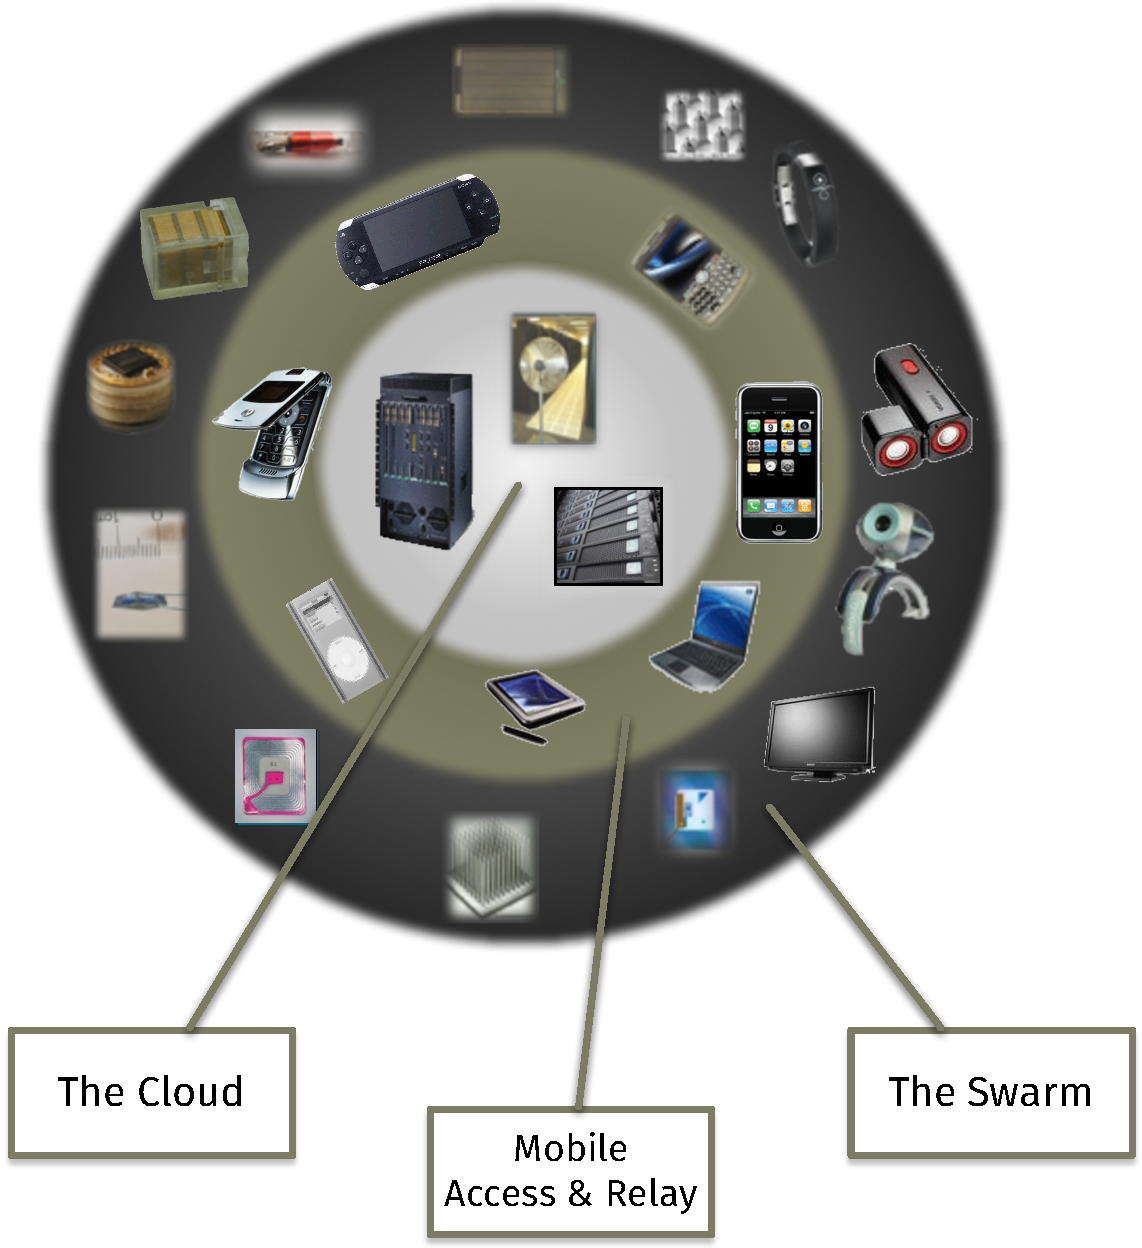
\includegraphics[width=0.8\textwidth]{figures/swarm_jan.pdf}
      \caption{J.\,Rabaey, ASPDAC'08}
    \end{figure}

    \pause

    \column{0.5\textwidth}
    Swarm, or
    \begin{itemize}
    \item \alert<4>{Internet of Things (IoT)}
    \item Internet of Everything (IoE)
    \item Industry 4.0
    \item The Industrial Internet
    \item TSensors (Trillion Sensors)
    \item Machine to Machine (M2M)
    \item Smarter Planet
    \end{itemize}

  \end{columns}
  \pause
  \begin{figure}
    
\includegraphics[width=\textwidth]{figures/swarmlogo.pdf}
  \end{figure}
\end{frame}

\begin{frame}{Gartner Hype Cycle (2015)}
  \begin{figure}
    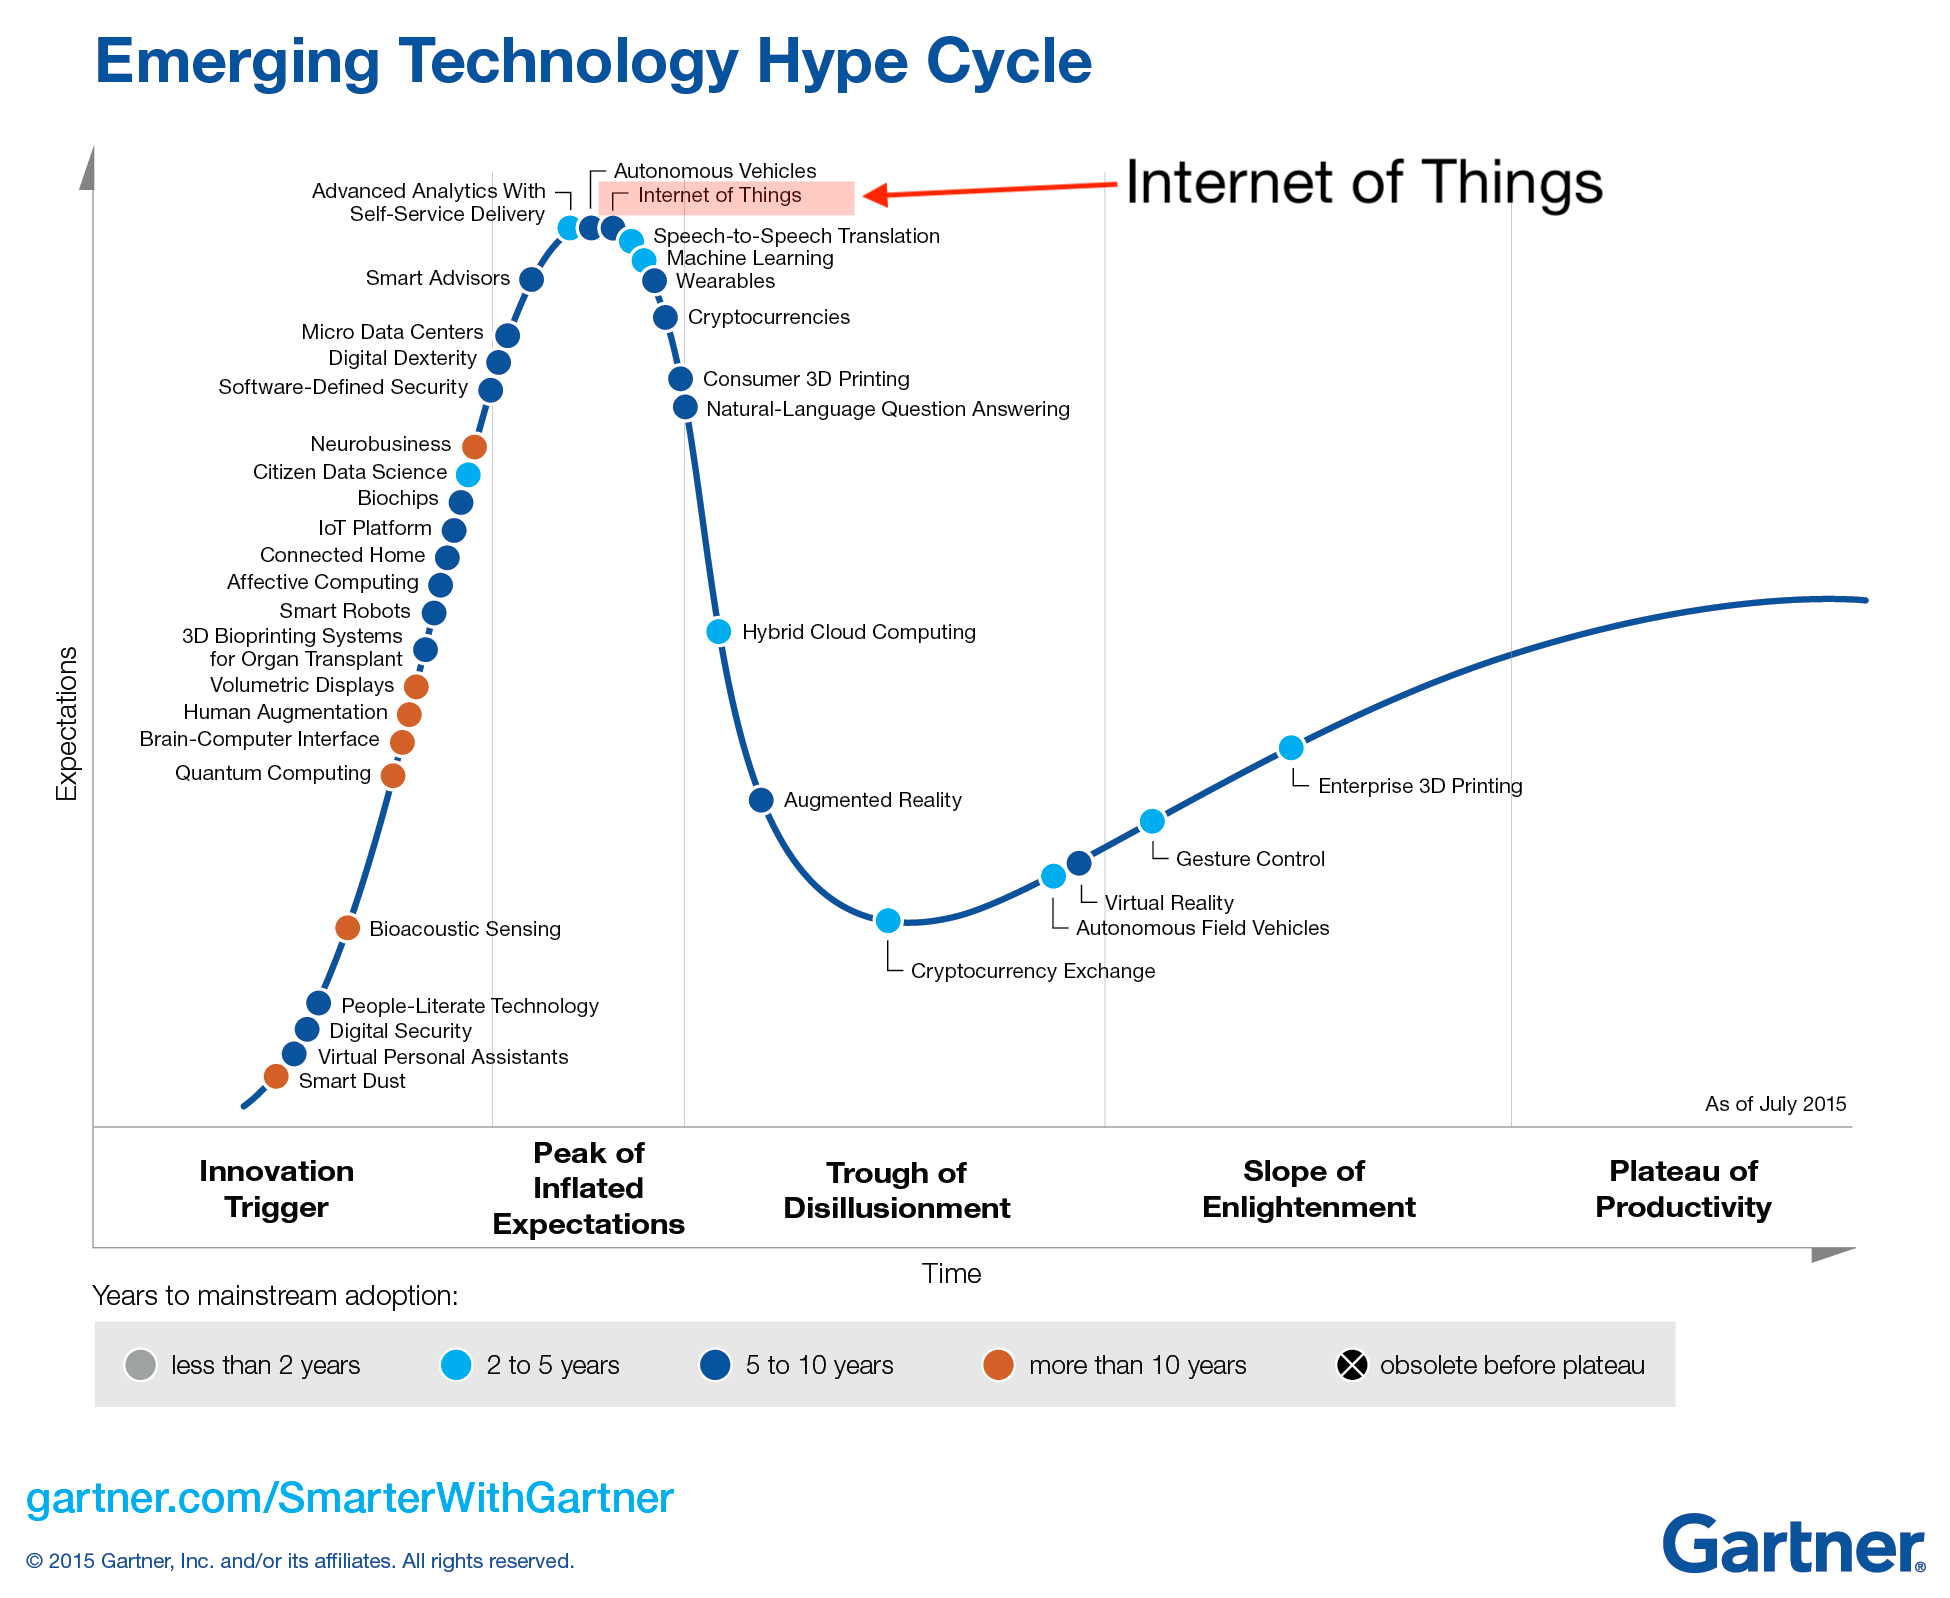
\includegraphics[width=0.8\textwidth]{figures/hype.png}
  \end{figure}
\end{frame}

\begin{frame}{A Cloud-centric Approach}
  \vspace{1em}
  \begin{figure}
    \centering
    \begin{subfigure}[t]{0.48\textwidth}
      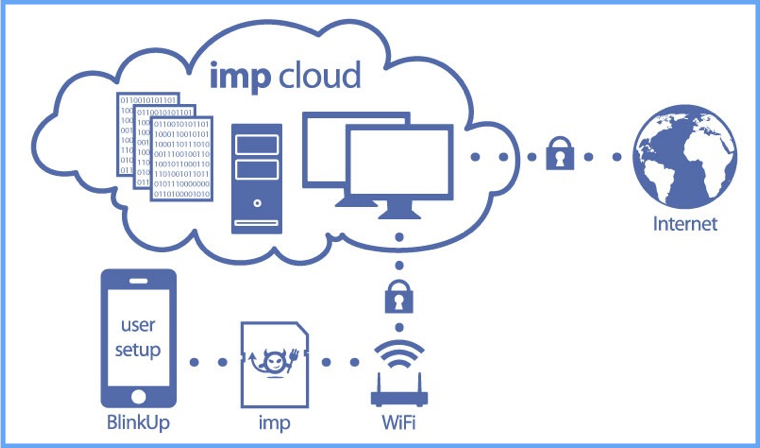
\includegraphics[width=\textwidth]{figures/cloud1.png}
      \caption{\href{http://www.limetrace.co.uk/electric-imp-platform}{Electric
          Imp}}
    \end{subfigure}
    \hfill
    \begin{subfigure}[t]{0.48\textwidth}
      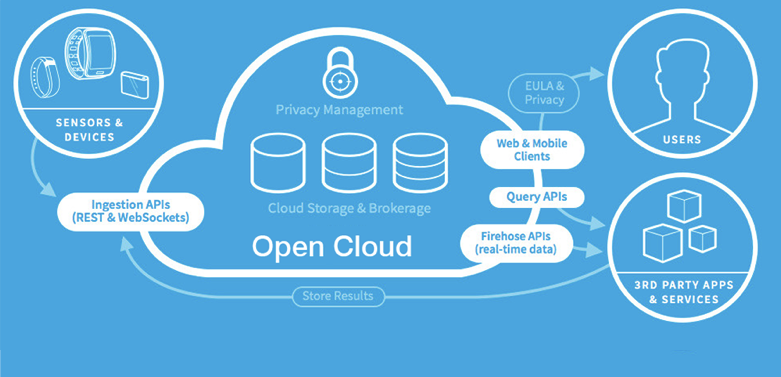
\includegraphics[width=\textwidth]{figures/cloud2.png}
      \caption{\href{https://developer.samsungsami.io/sami/sami-documentation/}{Samsung
          SAMI}}
    \end{subfigure}
    \begin{subfigure}[t]{0.7\textwidth}
      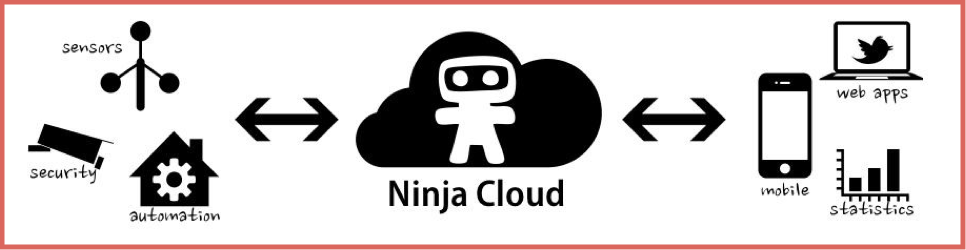
\includegraphics[width=\textwidth]{figures/cloud3.png}
      \caption{\href{http://lucept.files.wordpress.com/2012/06/ninja-blocks-capture.jpg}{Ninja Sphere}}
    \end{subfigure}
  \end{figure}
\end{frame}

\begin{frame}{``The Cloud'': Model vs.\,Reality}
  \begin{figure}
    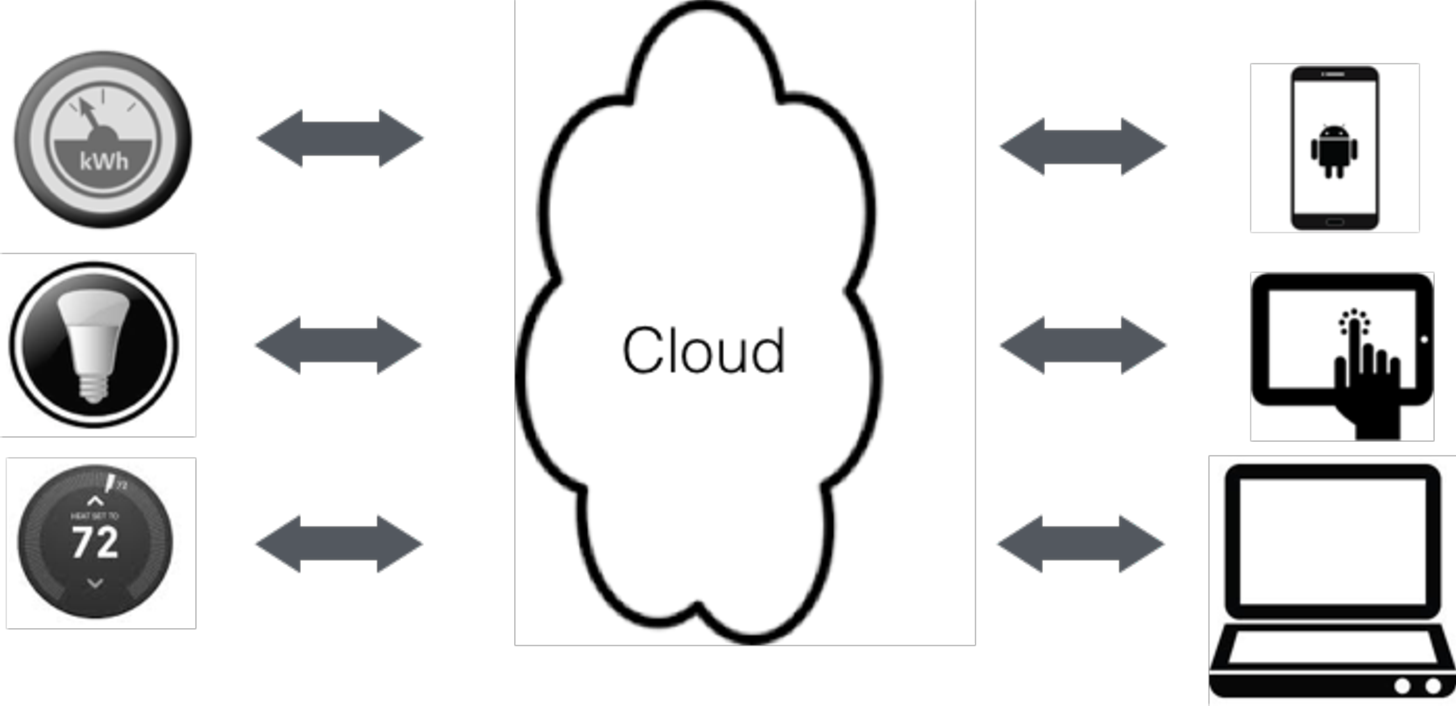
\includegraphics[width=0.6\textwidth]{figures/cloud-view.pdf}
  \end{figure}
  \vspace{-3em}
  \pause
  \begin{figure}
    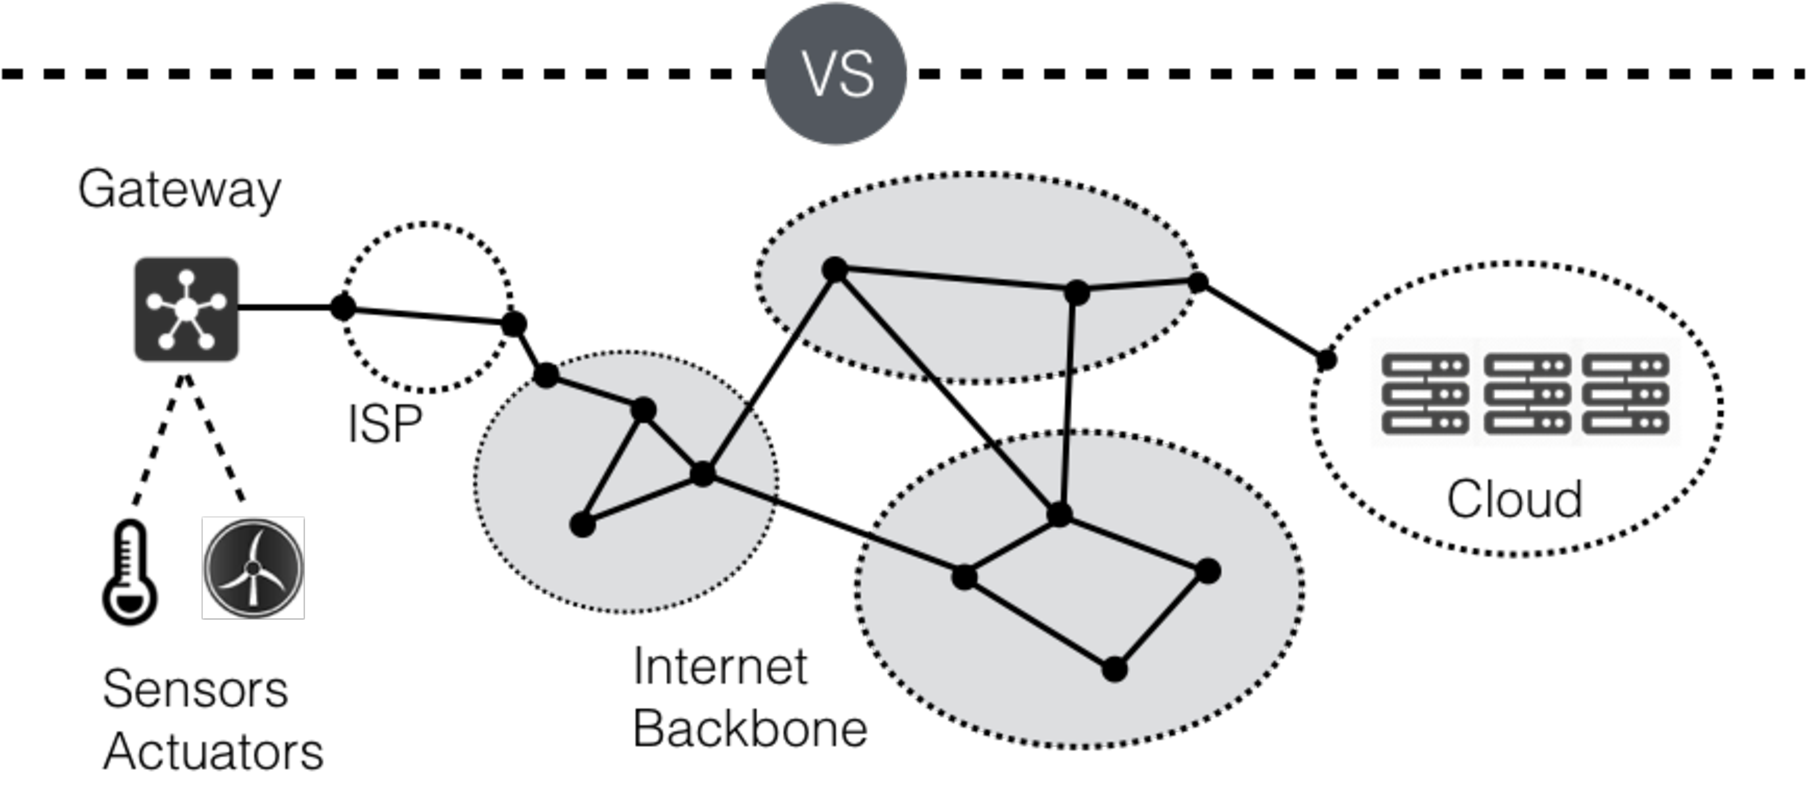
\includegraphics[width=0.7\textwidth]{figures/cloud-reality.pdf}
  \end{figure}
\end{frame}

\begin{frame}{The Cloud is Not Enough}
  \only<1>{
    \begin{table}
      \centering
      \begin{tabular}{c c c}
        \toprule
        & Web/IT & Swarm/IoT \\
        \midrule
        Privacy \& Security & Open for access & Sensitive data \\
        Scalability & Power law & Billion devices \\
        Interaction Model & Human & Machine \\
        Latency & Variable & Bounded  \\
        Bandwidth & Downstream & Upstream   \\
        Availability (QoS) & No guarantee & Requirement  \\
        Durability Management & Cloud controls & Users control \\
        \bottomrule
      \end{tabular}
      \caption{Pitfalls with Today’s Approach to IoT~\cite{zhang2015cloud}}
    \end{table}
  }
  \only<2>{
    \begin{table}
      \centering
      \begin{tabular}{c c c}
        \toprule
        & Web/IT & Swarm/IoT \\
        \midrule
        Privacy \& Security & Open for access & Sensitive data \\
        Scalability & Power law & Billion devices \\
        Interaction Model & Human & Machine \\
        \rowcolor{blue!30} Latency & Variable & Bounded  \\
        \rowcolor{blue!30} Bandwidth & Downstream & Upstream   \\
        Availability (QoS) & No guarantee & Requirement  \\
        Durability Management & Cloud controls & Users control \\
        \bottomrule
      \end{tabular}
      \caption{Pitfalls with Today’s Approach to IoT~\cite{zhang2015cloud}}
    \end{table}
  }
\end{frame}

\begin{frame}{Bandwidth: Downstream vs.\,Upstream}
  \vspace{1em}
  \begin{figure}
    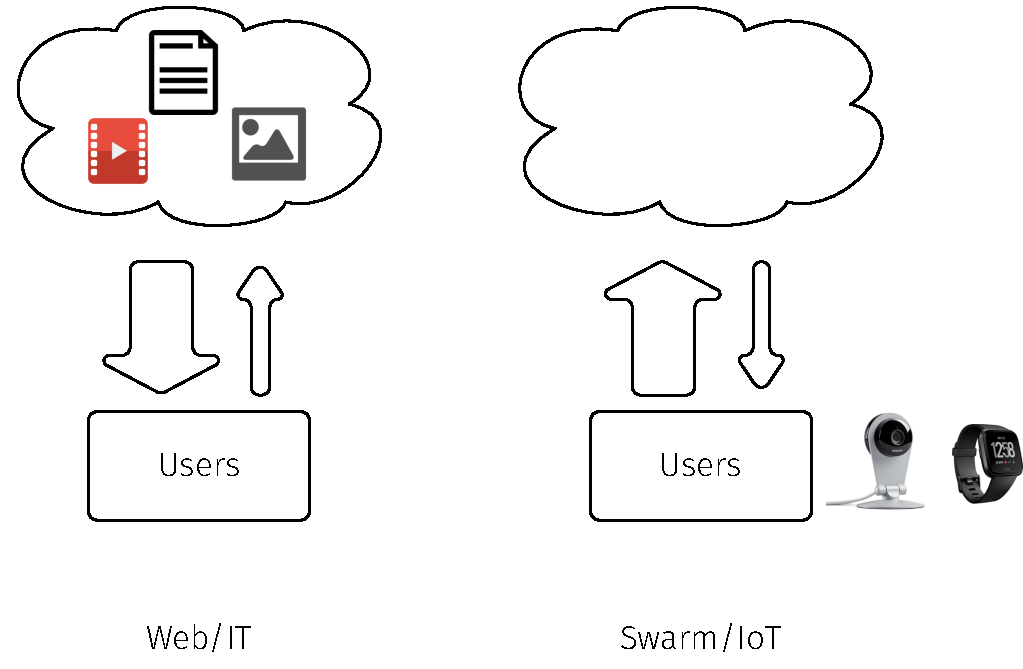
\includegraphics[width=0.9\textwidth]{figures/uplink-downlink.pdf}
  \end{figure}
\end{frame}

%%% Local Variables:
%%% mode: latex
%%% TeX-engine: xetex
%%% TeX-master: "talk"
%%% End:

\section{AWStream}

\begin{frame}{Fidelity vs.\,Freshness}
  \begin{figure}
    \centering
    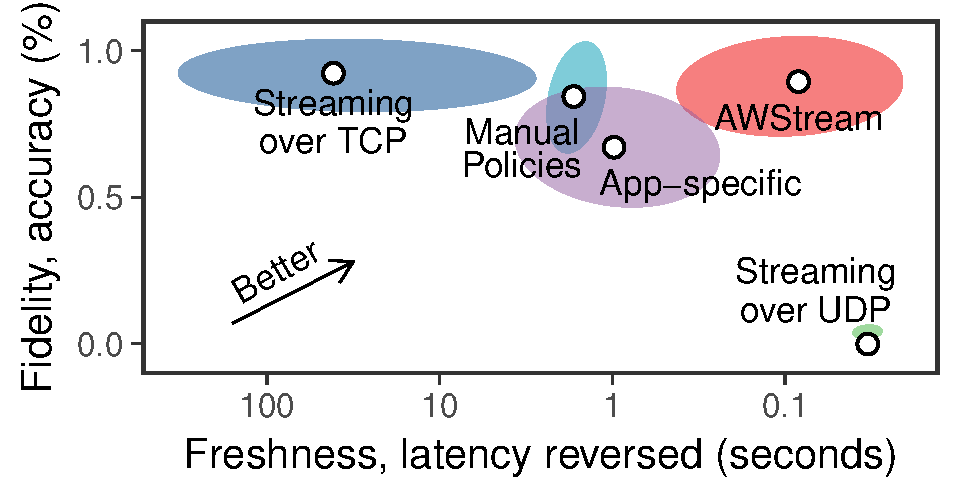
\includegraphics[width=0.8\columnwidth]{figures/fidelity-freshness.pdf}
    \caption{The trade-off space between data freshness and fidelity when facing
      insufficient bandwidth.}
  \end{figure}
\end{frame}

%%% Local Variables:
%%% mode: latex
%%% TeX-master: "talk"
%%% End:

\section{BRT}

\begin{frame}{Bounded Response Times}

\end{frame}

%%% Local Variables:
%%% mode: latex
%%% TeX-master: "../talk"
%%% End:

\begin{frame}{Summary and Contributions}
  \begin{itemize}
  \item Swarm/IoT has huge potentials but also challenges.
  \item Network resource adaptation
    \begin{itemize}
    \item Addresses scarce and limited WAN bandwidth.
    \item Tradeoff between application accuracy and data size demand.
    \end{itemize}
  \item Compute resource adaptation
    \begin{itemize}
    \item Addresses heterogeneous platforms and large parameter space.
    \item Tradeoff between application accuracy and processing times.
    \end{itemize}
  \item Overall, a systematic and quantitative approach for adaptation.
  \end{itemize}
\end{frame}

\begin{frame}{Current (other) and Future Work}
  \footnotesize

  \vspace{1em}
  \metroset{block=fill}
  \begin{block}{TerraSwarm Vision}
    TerraSwarm applications are characterized by their ability to
    \alert{dynamically recruit} resources such as sensors and data from the
    cloud, aggregate and use that information to make or aid decisions.
  \end{block}

  \pause
  
  \begin{figure}
    \begin{subfigure}{0.49\textwidth}
      \centering
      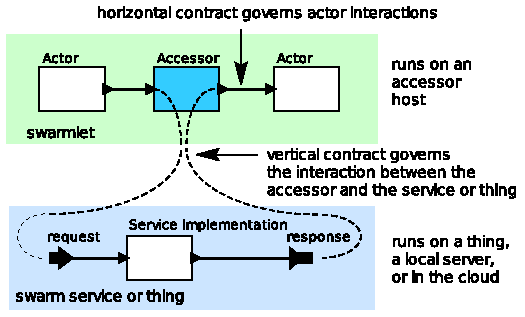
\includegraphics[height=0.4\textheight]{figures/accessors.pdf}
      \caption{Accessor in a network of actors.}
    \end{subfigure}
    \hfill
    \begin{subfigure}{0.49\textwidth}
      \centering
      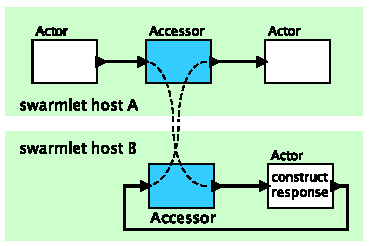
\includegraphics[height=0.4\textheight]{figures/accessors2.pdf}
      \caption{Instantiate accessors on another host.}
    \end{subfigure}
  \end{figure}

  \pause

  Work in progress with Marten and Andr\'es. Maybe checkout
  Marten's dissertation talk in the future :)
\end{frame}

%%% Local Variables:
%%% mode: latex
%%% TeX-master: "../talk"
%%% TeX-engine: xetex
%%% End:


\appendix

\begin{frame}[standout]
  Epilogue
\end{frame}

\section{Epilogue}

\begin{frame}{Lessons \& Philosophy: Adaptation in Life}
  \centering
  \vspace{3em}
  \begin{tikzpicture}
    \draw [thick] [<->] (0,6) node [left] {Happiness}
    -- (0,0) --
    (6,0) node [below] {Money};

    \foreach \Point in {(5.5, 5.5), (5, 5.2), (4.5, 4.9), (4, 4.5), (3.8, 4.3)}{
      % \node<+-> [ACMBlue] at \Point {x};
      \node [ACMBlue] at \Point {x};
    }
  \end{tikzpicture}
\end{frame}

\begin{frame}{Acknowledgment}

  \begin{figure}
    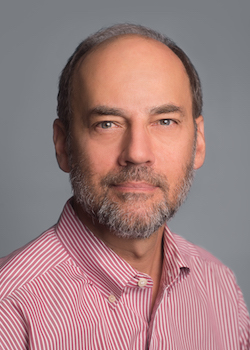
\includegraphics[width=0.15\linewidth]{figures/lee.jpg}
    \pause
    \hfill
    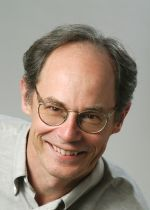
\includegraphics[width=0.15\linewidth]{figures/wawrzynek.jpg}
    \hfill
    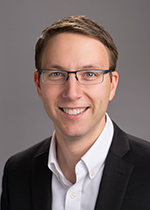
\includegraphics[width=0.15\linewidth]{figures/hartmann.jpg}
    \hfill
    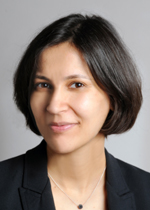
\includegraphics[width=0.15\linewidth]{figures/ratnasamy.jpg}
    \hfill
    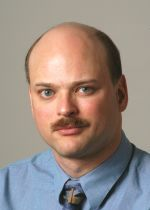
\includegraphics[width=0.15\linewidth]{figures/kubiatowicz.jpg}
    \hfill
  \end{figure}

  \begin{columns}
    \column{0.15\textwidth}
    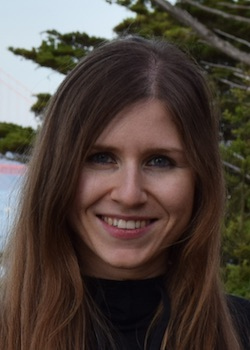
\includegraphics[width=0.9\linewidth]{figures/akkaya.jpg}
    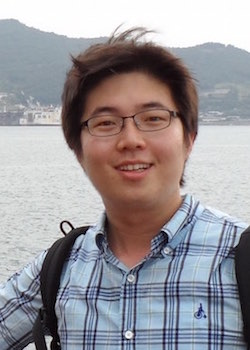
\includegraphics[width=0.9\linewidth]{figures/kim.jpg}

    \column{0.15\textwidth}
    
\includegraphics[width=0.9\linewidth]{figures/shaver.jpg}
    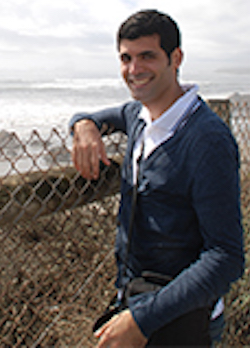
\includegraphics[width=0.9\linewidth]{figures/iannopollo.jpg}

    \column{0.7\textwidth}
    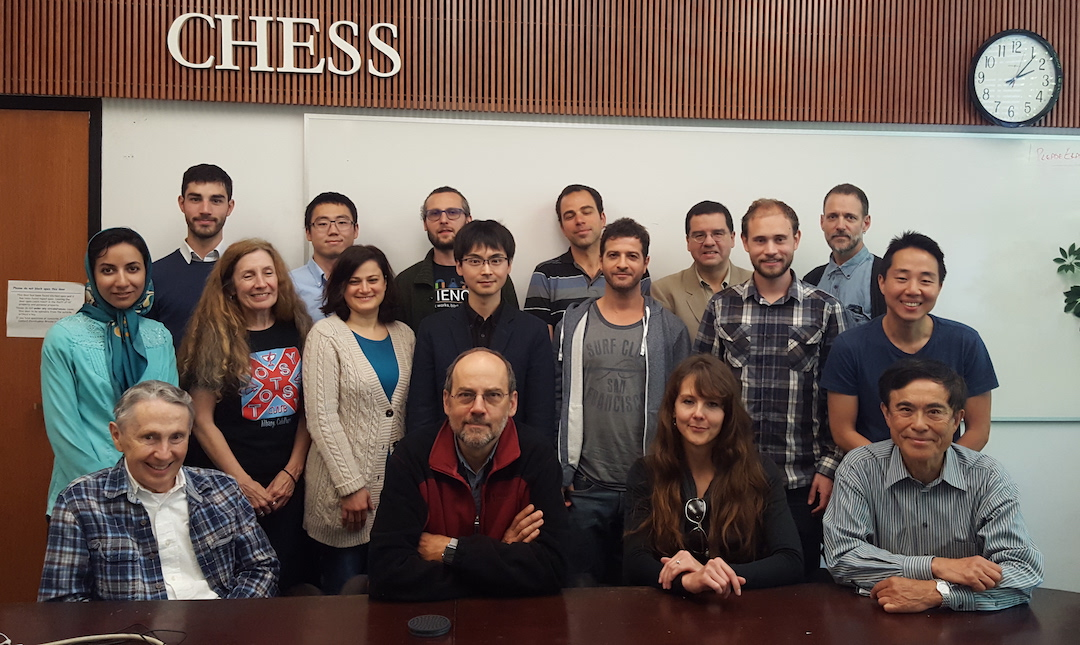
\includegraphics[width=0.9\linewidth]{figures/ptolemy_group.jpg}
  \end{columns}

\end{frame}

\begin{frame}{Acknowledgement}
  \footnotesize \textcolor{ACMRed}{\heartpar{Edward Lee, John Wawrzynek, Syliva
      Ratnasamy, John Chuang, Bj\"orn Hartmann, John Kubiatowicz, Lin Zhang,
      David Mellis, Xin Jin, Mary Stewart, Christopher Brooks, Eunsuk Kang, Ilge
      Akkaya, Hokeun Kim, Marten Lohstroh, Matt Weber, Antonio Iannopollo,
      Mehrdad Niknami, Chris Shaver (Yvan Vivid), Michael Zimmer, Christos
      Stergiou, Dai Bui, Ben Lickly, Eleftherios Matsikoudis, Joseph Ng, Chadlia
      Jerad Ep Ben Haj Hmida, Moez Ben Haj Hmida, Maryam Bagheri, Victor
      Nouvellet, Ankush Desai, Nitesh Mor, Yu-Hsiang Sean Chen, Claire Tuna,
      Achal Dave, Jack Kolb, Eric Allman, Roy Wang, Bill N. Schilit, Jin Liang,
      Chao Mei, Kaifei Chen, Qifan Pu, Xiang Gao, Peihan Miao, Zhuo Chen, Yuting
      Wei, Chaoran Guo, Qian Zhong, Tianshi Wang}}
\end{frame}

%%% Local Variables:
%%% mode: latex
%%% TeX-master: "talk"
%%% TeX-engine: xetex
%%% End:


\begin{frame}[standout]
  Backup Slides.
\end{frame}

\begin{frame}{Video Encoding Frames}
  \begin{figure}
    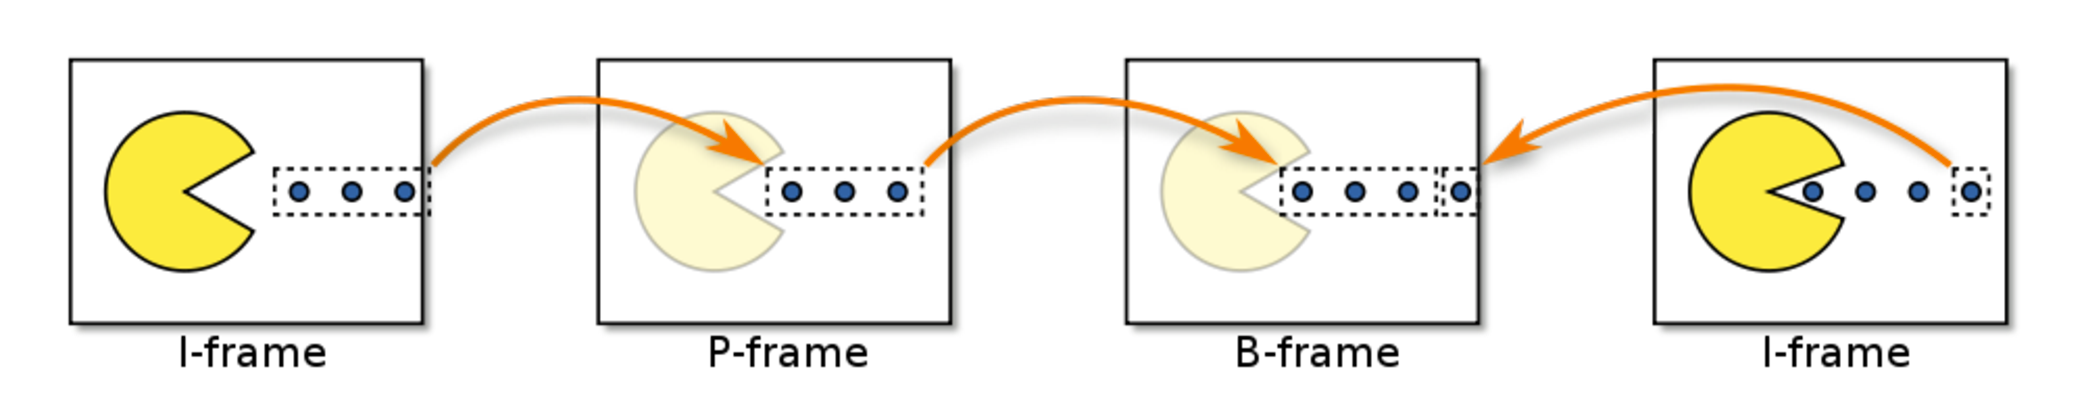
\includegraphics[width=\textwidth]{figures/video-frames.pdf}
    \caption{PC: https://en.wikipedia.org/wiki/Video\_compression\_picture\_types}
  \end{figure}

  \begin{itemize}
  \item \textbf{I-frames} are the least compressible but don't require other
    video frames to decode. I-frames are further compressed with
    quantization.
  \item \textbf{P-frames} can use data from previous frames to decompress
    and are more compressible than I-frames.
  \item \textbf{B-frames} can use both previous and forward frames for data
    reference to get the highest amount of data compression (not an option
    in live streaming).
  \end{itemize}
\end{frame}

\begin{frame}{Evaluation: Resource Allocation for Multiple Applications}
  \centering
  \begin{figure}
    \centering
    \begin{subfigure}[t]{0.7\columnwidth}
      \centering
      
\includegraphics[width=\textwidth]{figures/multitask-legend.pdf}
    \end{subfigure}
    \\
    \vspace{1em}
    \begin{subfigure}[t]{0.45\columnwidth}
      \centering
      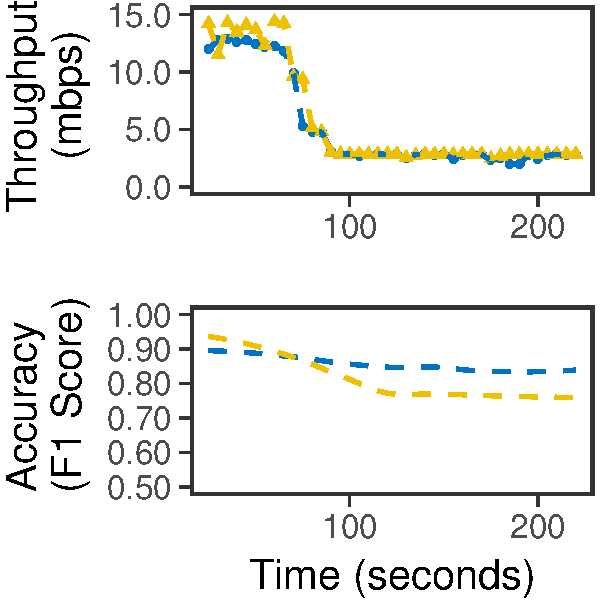
\includegraphics[width=\textwidth]{figures/multitask-left.pdf}
      \caption{Resource Fairness}
      \label{fig:eq-bw}
    \end{subfigure}
    \hfill
    \begin{subfigure}[t]{0.45\columnwidth}
      \centering
      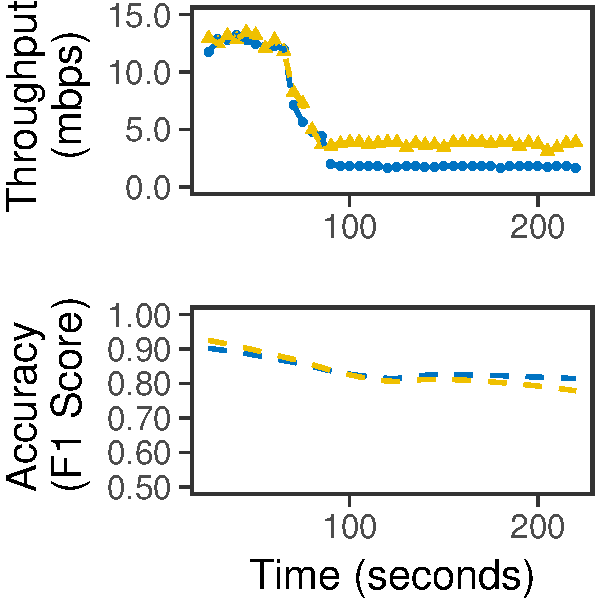
\includegraphics[width=\textwidth]{figures/multitask-right.pdf}
      \caption{Utility Fairness}
      \label{fig:eq-acc}
    \end{subfigure}
  \end{figure}
\end{frame}

\begin{frame}{Bandwidth Fluctuations (Cellular)}
  \hypertarget{cellular-variation}{}
  \begin{figure}
    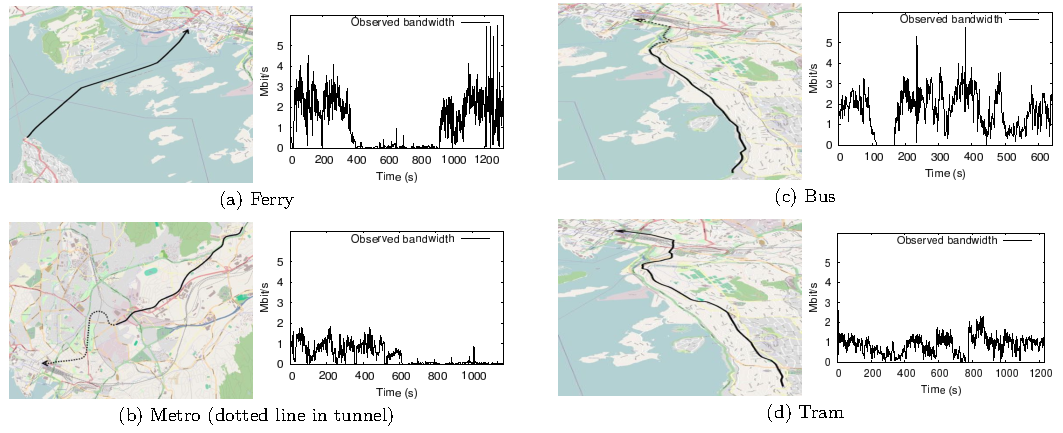
\includegraphics[width=\textwidth]{figures/bandwidth-cellular.pdf}
    \caption{Riiser, Haakon, et al. "A comparison of quality scheduling in
      commercial adaptive HTTP streaming solutions on a 3G network."
      Proceedings of the 4th Workshop on Mobile Video. ACM, 2012.}
  \end{figure}
\end{frame}

\begin{frame}{Bandwidth Fluctuations (WiFi)}
  \footnotesize
  \begin{figure}
    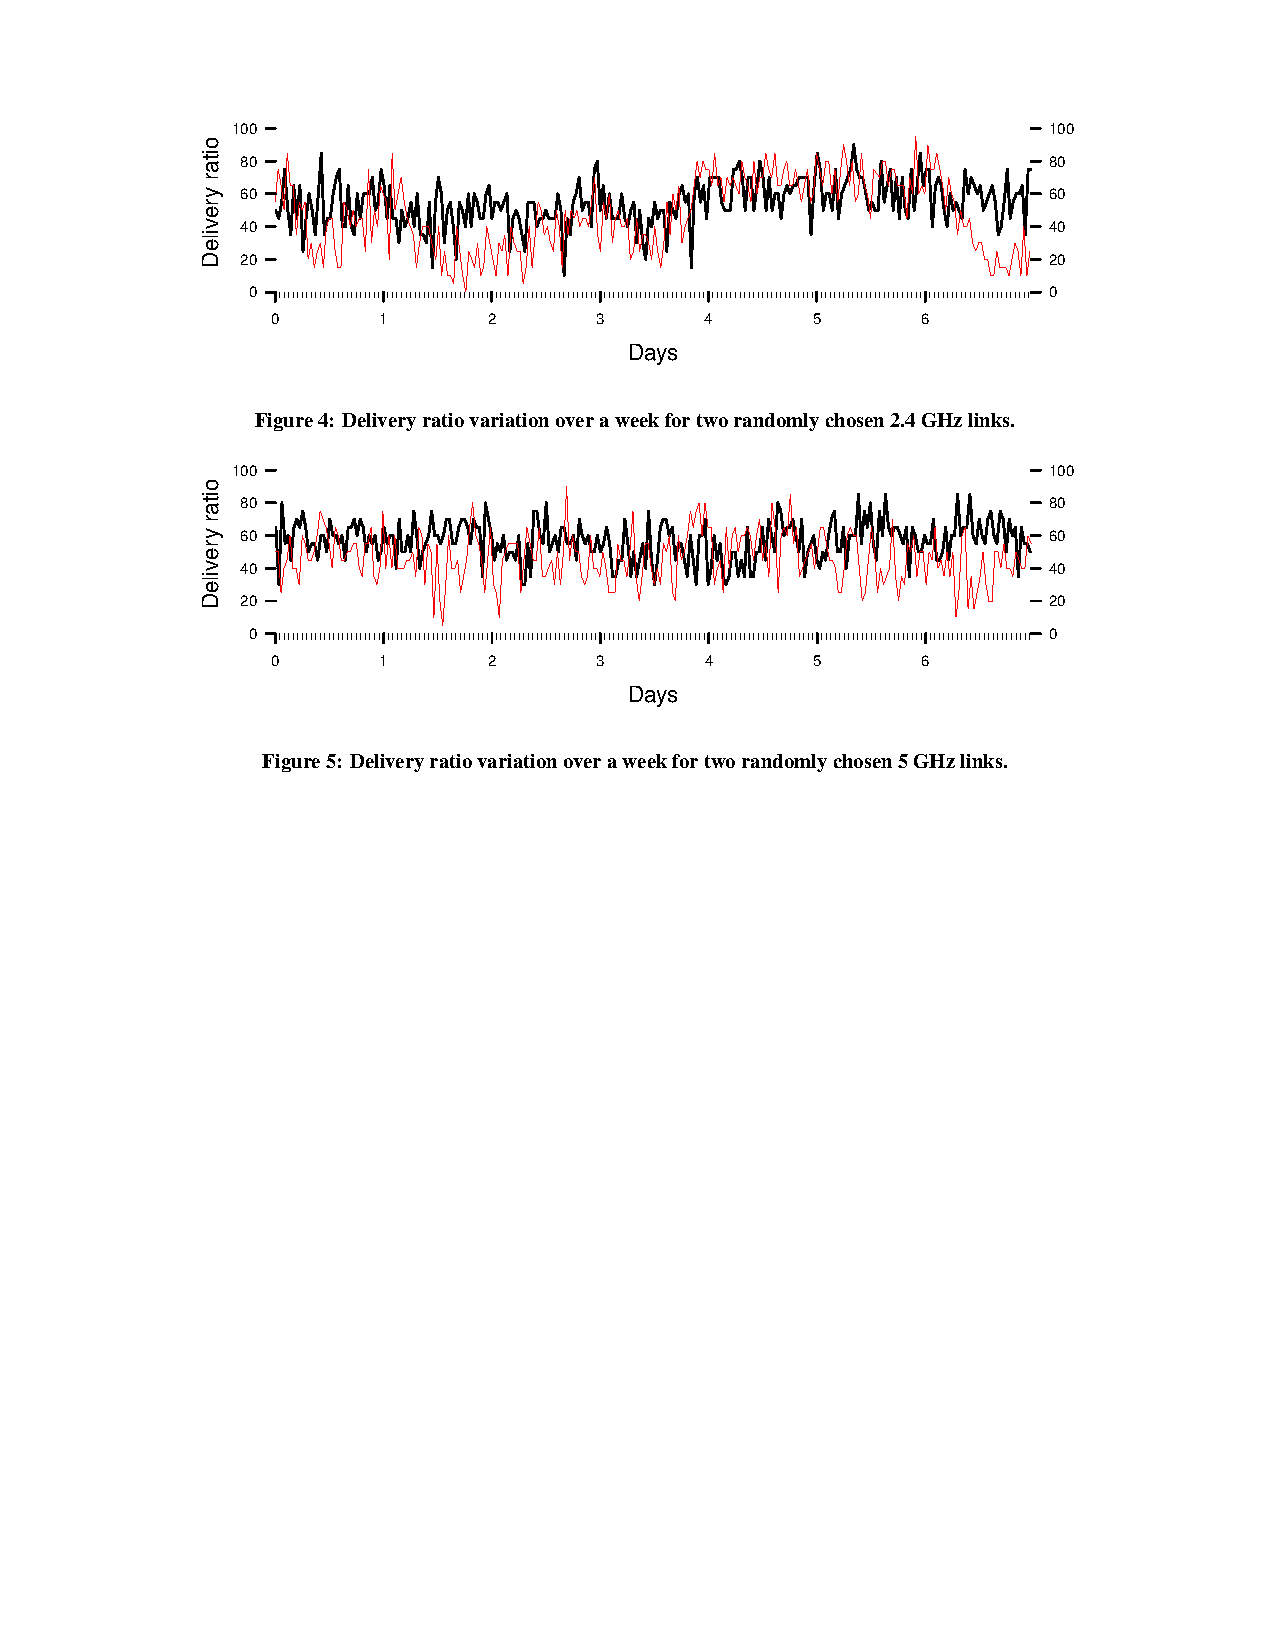
\includegraphics[width=0.7\textwidth]{figures/bandwidth-wifi.pdf}
    \caption{Biswas et al, Cisco Meraki, Large-scale Measurements of Wireless
      Network Behavior, SIGCOMM'15. Two randomly chosen links.}
  \end{figure}

  \hyperlink{aws-variation}{Continue with the main slides}.
\end{frame}

\begin{frame}{Augmented Reality}
  \begin{itemize}
  \item Training and testing data characteristics
    \begin{itemize}
    \item 1920x1080 resolution with 30 FPS
    \item training: 707 frames (23.5 seconds), testing: 1384 frames (46 seconds)
    \end{itemize}
  \item Object Recognition
    \begin{itemize}
    \item Darknet: Open Source Neural Networks in C
    \item Developed by Joseph Redmon, "Do whatever you want with it" license
    \item It supports CPU/GPU
    \item In this work, I am using a pre-trained model with Coco dataset
    \end{itemize}
  \item Other systems such as TensorFlow, Caffe would also work
  \end{itemize}
\end{frame}

\begin{frame}{IOU and F1}
  \hypertarget{iou-f1}{}
  \vspace{1em}
  \begin{columns}
    \column{0.5\textwidth}
    Positive if intersection over union (IOU) larger than 0.5.

    \[
      \text{IOU} = \frac{\text{Area of Intersection}}{\text{Area of Union}}
    \]

    \begin{figure}
      \begin{subfigure}{0.3\textwidth}
        \begin{tikzpicture}
          \fill[color=blue!30] (0.5, 0.5) rectangle (1, 1);
          \node[draw=none] () at (1.5, 1.5) {};
          \draw (0, 0) rectangle (1, 1);
          \draw[densely dashed] (0.5, 0.5) rectangle (1.5, 1.5);
        \end{tikzpicture}
        \caption{IOU=0.14}
      \end{subfigure}
      \begin{subfigure}{0.3\textwidth}
        \begin{tikzpicture}
          \fill[color=blue!30] (0.15, 0.15) rectangle (1, 1);
          \node[draw=none] () at (1.5, 1.5) {};
          \draw (0, 0) rectangle (1, 1);
          \draw[densely dashed] (0.15, 0.15) rectangle (1.15, 1.15);
        \end{tikzpicture}
        \caption{IOU=0.57}
      \end{subfigure}
      \begin{subfigure}{0.3\textwidth}
        \begin{tikzpicture}
          \fill[color=blue!30] (0.05, 0.05) rectangle (1, 1);
          \node[draw=none] () at (1.5, 1.5) {};
          \draw[densely dashed] (0.05, 0.05) rectangle (1.05, 1.05);
          \draw (0, 0) rectangle (1, 1);
        \end{tikzpicture}
        \caption{IOU=0.82}
      \end{subfigure}
    \end{figure}

    \column{0.5\textwidth}
    
    F1 is the harmonic mean of precision and recall:

    \begin{table}
      \centering
      \begin{tabular}{| c | c | c |}
        \hline
        & P & N \\
        \hline
        Y & True Positive & False Positive \\
        \hline
        N & True Positive & False Positive \\
        \hline
      \end{tabular}
    \end{table}

    \begin{equation*}
      \begin{split}
        \text{Precision} &= \frac{\text{true positive}}{\text{all positive}} \\
        \text{Recall} &= \frac{\text{true positive}}{\text{all detection}} \\
        \text{F1} &= \frac{2}{\frac{1}{\text{Recall}} + \frac{1}{\text{Precision}}}
      \end{split}
    \end{equation*}
  \end{columns}
\end{frame}

%%% Local Variables:
%%% mode: latex
%%% TeX-master: "talk"
%%% TeX-engine: xetex
%%% End:


\else

% \begin{frame}{(1) Stream Processing APIs}
  \vspace{1em}
  \centering
  \begin{tikzpicture}
    \node[bn, minimum width=2cm] (op) {Operator};
    \node [left=1cm of op] (left) {Data Stream};
    \node [right=1cm of op] (right) {Data Stream};
    \draw[to] (left) -- (op);
    \draw[to] (op) -- (right);
  \end{tikzpicture}

  \visible<2->{
    \vspace{1em}
    \scalebox{0.7}{
      \begin{tikzpicture}
        \node[bn, minimum width=3cm] (op) {map(f)};
        \node [left=1cm of op] (left) {$\{x_1, x_2, x_3, x_4, \ldots \}$};
        \node [right=1cm of op] (right) {$\{f(x_1), f(x_2), f(x_3), f(x_4), ...\}$};
        \draw[to] (left) -- (op);
        \draw[to] (op) -- (right);

        \node[bn, minimum width=3cm, below=0.5cm of op] (op2) {window(2, f)};
        \node [left=1cm of op2] (left2) {$\{x_1, x_2, x_3, x_4, \ldots \}$};
        \node [right=1cm of op2] (right2) {$\{f(x_1, x_2), f(x_3, x_4), ...\}$};
        \draw[to] (left2) -- (op2);
        \draw[to] (op2) -- (right2);

        \visible<4->{
        \node[bn, minimum width=3cm, below=0.5 of op2] (op3) {maybe($\vec{k}$, f)};
        \node [left=1cm of op3] (left3) {$\{x_1, x_2, x_3, x_4, \ldots \}$};
        \node [right=1cm of op3] (right3) {$\{f(x_1, k_{i_1}), f(x_2, k_{i_2}), f(x_3, k_{i_3}),
          f(x_4, k_{i_4}), ...\}$};
        \draw[to] (left3) -- (op3);
        \draw[to] (op3) -- (right3);
        }
      \end{tikzpicture}
    }
  }
  
  \visible<3->{
  \begin{table}
    \scriptsize
    \begin{tabular}{ c r l }
      \toprule
      \multirow{4}{*}{Normal}
      & \textit{map} (f: I $\Rightarrow$ O) & Stream<I> $\Rightarrow$ Stream<O> \\
      & \textit{skip} (i: Integer) & Stream<I> $\Rightarrow$
                                     Stream<I> \\
      & \textit{window} (count: Integer, f: Vec<I> $\Rightarrow$ O) & Stream<I> $\Rightarrow$
                                                                      Stream<O> \\
      & ... & ... \\
      \midrule \visible<5->{
      \multirow{4}{*}{Adaptation}
      & \textit{maybe} (knobs: Vec<T>, f:  (T, I) $\Rightarrow$ I) & Stream<I> $\Rightarrow$
                                                                     Stream<I> \\
      & \textit{maybe\_skip} (knobs: Vec<Integer>) & Stream<I> $\Rightarrow$ Stream<I> \\
      & \textit{maybe\_head} (knobs: Vec<Integer>) & Stream<Vec<I>{}> $\Rightarrow$
                                                     Stream<Vec<I>{}> \\
      & ... & ... \\
      \bottomrule
      }
    \end{tabular}
  \end{table}
  }
\end{frame}

\begin{frame}[fragile]{\texttt{maybe(knobs: Vec<T>, f: (T, I) => I)}}
  \begin{tikzpicture}[
    level distance=2cm,
    level 1/.style={sibling distance=4cm},
    edge from parent/.style={->,draw},
    >=latex]
    \node[bn] {
\begin{lstlisting}
let quantized_stream = vec![1, 2, 3, 4].into_stream()
    .maybe(vec![2, 4], |k, val| val / k)
    .collect();
\end{lstlisting}
    }
    child {node[yn] (c1) {[1, 2, 3, 4]} edge from parent node [left] {no degradation}}
    child {node[yn] (c2) {[0, 1, 1, 2]} edge from parent node [left] {k = 2}}
    child {node[yn] (c3) {[0, 0, 0, 1]} edge from parent node [left] {k = 4}};
  \end{tikzpicture}

  \pause
  \vspace{2em}
  We rewrite the video streaming application as follows{\let\thefootnote\relax\footnote{{Example code in
    Rust, simplified for presentation.}}},

  \centering
  \begin{lstlisting}
let app = Camera::new((1920, 1080), 30)
    .maybe_downsample(vec![(1600, 900), (1280, 720)])
    .maybe_skip(vec![2, 5])
    .map(|frame| pedestrian_detect(frame))
    .compose();
  \end{lstlisting}
\end{frame}

%%% Local Variables:
%%% mode: latex
%%% TeX-master: "../talk"
%%% TeX-engine: xetex
%%% End:

% \begin{frame}[fragile]{(2) Profiling}
  \vspace{1em}
  \centering
  \begin{tikzpicture}
    \node[draw=none] (center) {};
    \node[bn, above=1cm of center] (code) {
\begin{lstlisting}
let app = Camera::new((1920, 1080), 30)
    .maybe_downsample(vec![(1600, 900), (1280, 720)])
    .maybe_skip(vec![2, 5])
    .map(|frame| pedestrian_detect(frame))
    .compose();
\end{lstlisting}
    };
    
    \visible<2->{
      \node[bn, minimum width=3.5cm, left=2cm of center] (data) {Training Data};
    }
    \visible<3->{
      \node[bn, minimum width=3.5cm, right=2cm of center] (func) {Accuracy
        Function};
    }
    
    \visible<4->{
      \node[draw=none, below=1cm of center] (target) {};
      \node[draw=none, left=0.2cm of target] (targeta) {};
      \node[draw=none, right=0.2cm of target] (targetb) {};
      \draw[to] (code) -- (target);
      \draw[to] (data) -- (targeta);
      \draw[to] (func) -- (targetb);
    }
  \end{tikzpicture}

  \visible<4->{
  \vspace{-1em}
  \footnotesize
  \begin{table}
    \begin{tabular}{c c c c}
      \toprule
      downsample & skip & bandwidth & accuracy \\
      \midrule
      (1920, 1080) & 0 & 10.7 & 1.0 \\
      (1600, 900)  & 0 & 8.3 & 0.88  \\
      (1280, 720)  & 0 & 6.3 & 0.87 \\
      (1920, 1080) & 2 & 9.3 & 0.90 \\
      ... & ... & ... & ... \\
      \bottomrule
    \end{tabular}
  \end{table}
  }
\end{frame}

\begin{frame}{Profile: Pareto-optimal Strategy}
  \begin{columns}
    \begin{column}{0.39\textwidth}
      \centering
      \only<1->{
      \begin{tikzpicture}
        \begin{axis}[
          width  = \textwidth,
          xlabel = Bandwidth (normalize),
          ylabel = Accuracy,
          ymin   = 0,
          ymax   = 1,
          ytick  = {0, 1},
          xmin   = 0,
          xmax   = 1,
          xtick  = {0, 1},
          ]

          \only<2->{
            \addplot[color=red, mark=x, only marks] coordinates {(0.95,0.95)};
          }
          \only<3->{
            \addplot[color=red, mark=x, only marks] coordinates {(0.90,0.92)};
          }
          \only<4->{
            \addplot[color=red, mark=x, only marks] coordinates {(0.85,0.90)};
          }
          \only<5->{
            \addplot[color=red, mark=x, only marks] coordinates {(0.70,0.80)};
          }
          \only<6->{
            \addplot[color=blue, mark=x, only marks] coordinates {(0.75,0.75)};
          }
          \only<7->{
            \addplot[color=red, mark=x, only marks] coordinates {
              (0.6, 0.7)
              (0.5, 0.65)
              (0.4, 0.55)
              (0.3, 0.50)
              (0.2, 0.45)
              (0.1, 0.20)
            };
            \addplot[color=blue, mark=x, only marks] coordinates {
              (0.83, 0.62)
              (0.80, 0.59)
              (0.74, 0.60)
              (0.63, 0.56)
              (0.61, 0.36)
              (0.51, 0.34)
              (0.50, 0.40)
              (0.49, 0.41)
              (0.47, 0.42)
              (0.46, 0.30)
              (0.44, 0.25)
              (0.24, 0.20)
              (0.10, 0.10)
            };
          }
          
        \end{axis}
      \end{tikzpicture}
      }
    \end{column}

    \begin{column}{0.59\linewidth}
      \scriptsize
      \begin{table}
        \centering
        \begin{tabular}{r l}
          \toprule
          \textbf{Symbol} & \textbf{Description} \\
          \midrule
          $n$ & number of degradation operations \\
          $k_i$ & the \textit{i}-th degradation knob \\
          $c = [k_{1}, k_{2}, ... k_{n}]$ & one specific configuration \\
          $\mathbb{C}$ & the set of all configurations \\
          \midrule
          $B(c)$ & bandwidth requirement for $c$ \\
          $A(c)$ & accuracy measure for $c$ \\
          $\mathbb{P}$ & Pareto-optimal set \\
          \bottomrule
        \end{tabular}
      \end{table}

      \visible<8->{
        \[
          \mathbb{P} = \{ c \in \mathbb{C} :
          \underbrace{\{ c' \in \mathbb{C}: B(c') < B(c),
            A(c') > A(c) \}}_{\text{set of better configurations $c'$}}
          = \varnothing\}
        \]

        See red markers in the figure.
      }
        
    \end{column}
  \end{columns}
\end{frame}

%%% Local Variables:
%%% mode: latex
%%% TeX-master: "../talk"
%%% TeX-engine: xetex
%%% End:

% \begin{frame}{Applications}
  \begin{table}
    \scriptsize
    \centering
    \begin{tabular}{c c c c}
      \toprule
      Application & Knobs & Accuracy & Dataset \\
      \midrule
      \specialcell{Augmented\\Reality}
                  & \specialcell{resolution \\ frame rate \\ quantization }
                  & \specialcell{F1 score\\\cite{Rijsbergen:1979:IR:539927}}
                  & \specialcell{iPhone video clips\\training: office (24s)\\testing: home (246s)} \\
      
      \midrule
      \specialcell{Pedestrian\\Detection}
                  & \specialcell{resolution \\ frame rate \\ quantization }
                  & F1 score
                          & \specialcell{MOT16~\cite{milan2016mot16}\\training: MOT16-04\\testing: MOT16-03} \\
      \midrule
      \specialcell{Log Analysis\\(Top-K, K=50)}
                  & \specialcell{head (N) \\ threshold (T) }
                  & \specialcell{Kendall's $\tau$\\\cite{abdi2007kendall}}
                  & \specialcell{\href{https://www.sec.gov}{SEC.gov} logs~\cite{edgarlog} \\ training: 4 days \\
      testing: 16 days} \\
      \bottomrule
    \end{tabular}
  \end{table}

  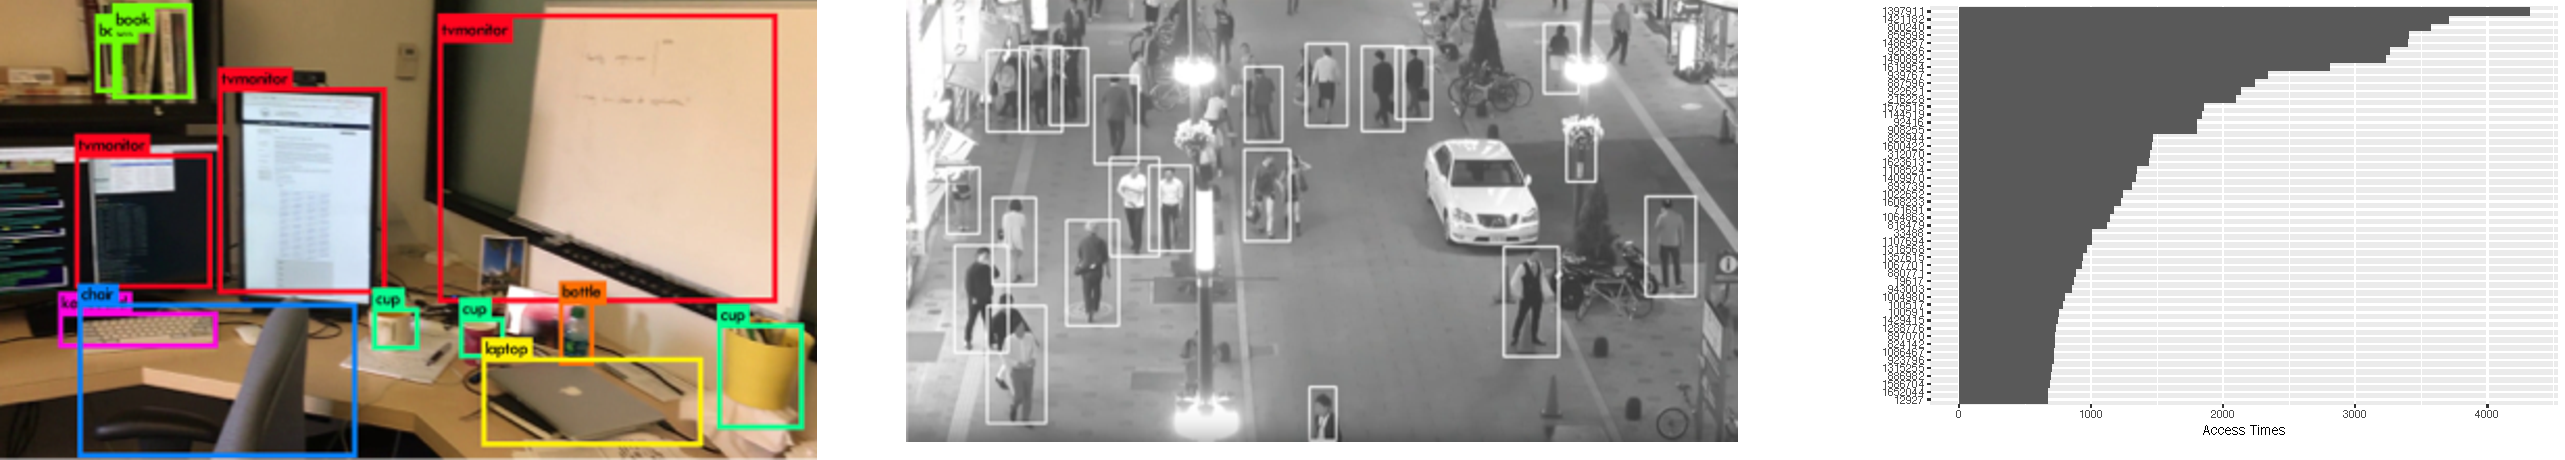
\includegraphics[width=\linewidth]{figures/apps.pdf}
\end{frame}

\begin{frame}{Top-K}
  \centering
  \begin{figure}
    \centering
    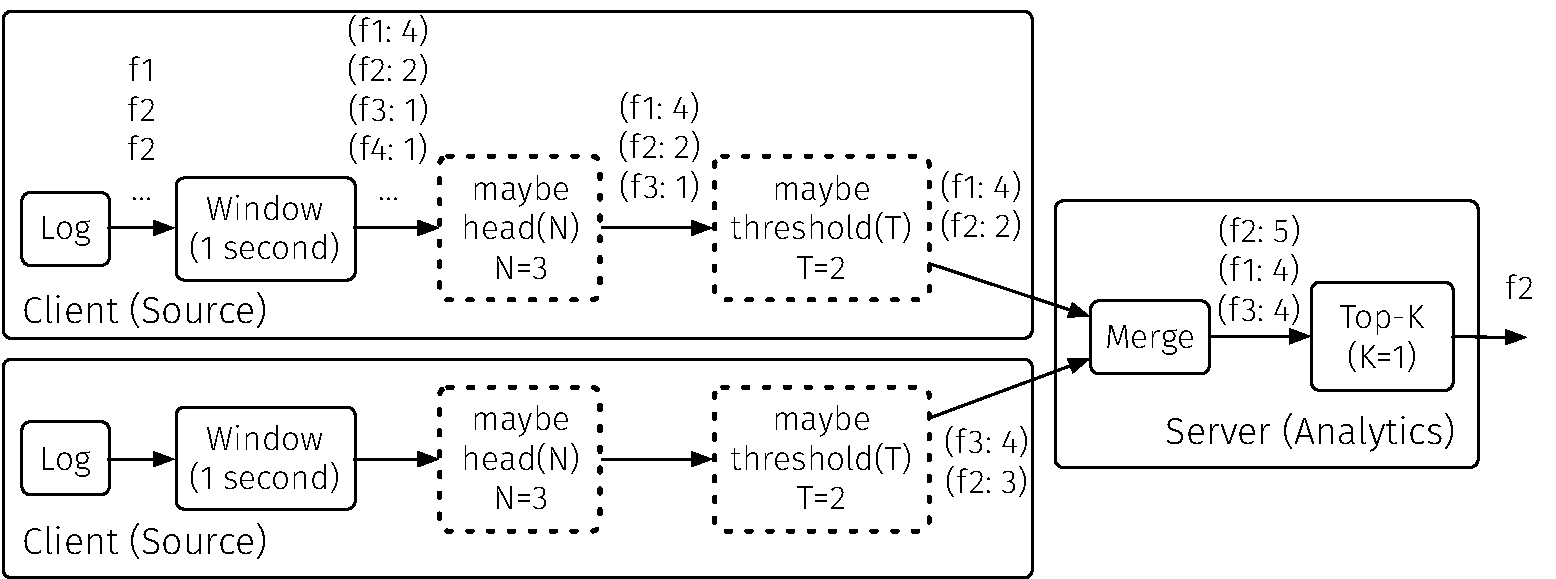
\includegraphics[width=\linewidth]{figures/topk.pdf}
    \caption{A distributed Top-K application with two degradation operations:
      \texttt{head} and \texttt{threshold}. In this example, \texttt{f2}, which
      is not in Top-1 for either client, becomes the global Top-1 after the
      merge. It would have been purged if the clients use threshold T=3,
      demonstrating degradation that reduces data sizes affects fidelity.}
    \label{fig:topk}
    \vspace{-0.5em}
  \end{figure}
\end{frame}

%%% Local Variables:
%%% mode: latex
%%% TeX-master: "../talk"
%%% TeX-engine: xetex
%%% End:

\begin{frame}{Evaluation: Generated Profiles}
  \begin{figure}
    \centering
    \begin{subfigure}[t]{0.48\textwidth}
      \centering
      \caption{Augmented Reality (AR)}
      \label{fig:ar-profile}
      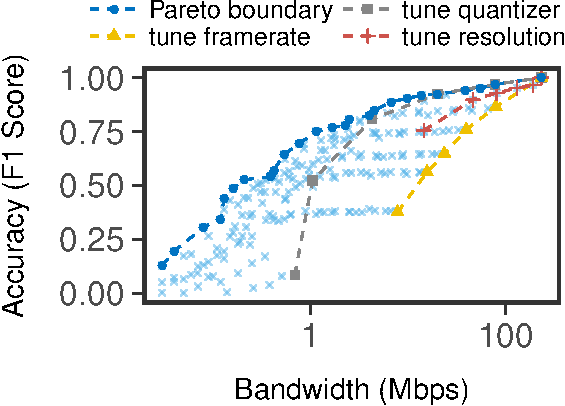
\includegraphics[width=\textwidth]{figures/profile-darknet.pdf}
    \end{subfigure}
    \hfill
    \begin{subfigure}[t]{0.48\textwidth}
      \centering
      \caption{Pedestrian Detection (PD)}
      \label{fig:pd-profile}
      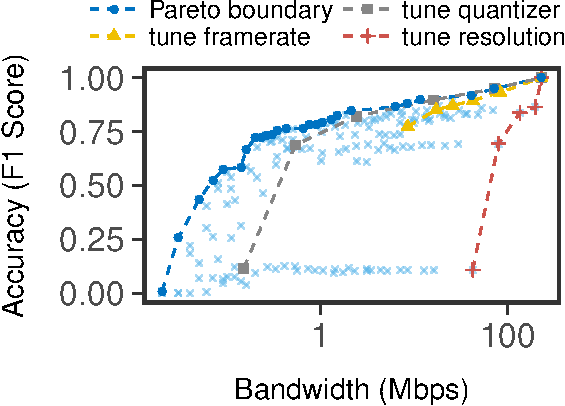
\includegraphics[width=\textwidth]{figures/profile-mot.pdf}
    \end{subfigure}
  \end{figure}

  \begin{itemize}
    \footnotesize
    \visible<2->{
    \item Optimal strategy is achieved with multiple dimensions; tuning one
      dimension leads to suboptimal performance.
    }
    \visible<3->{
    \item For the same application, different dimensions have different impact.
    }
    \visible<4->{\item For different applications, the same dimension has different
      impact.
    }
  \end{itemize}
\end{frame}

\begin{frame}{Evaluation: Generated Profiles (Top-K)}
  \begin{columns}
    \begin{column}{0.45\textwidth}
      \begin{figure}
        \centering
        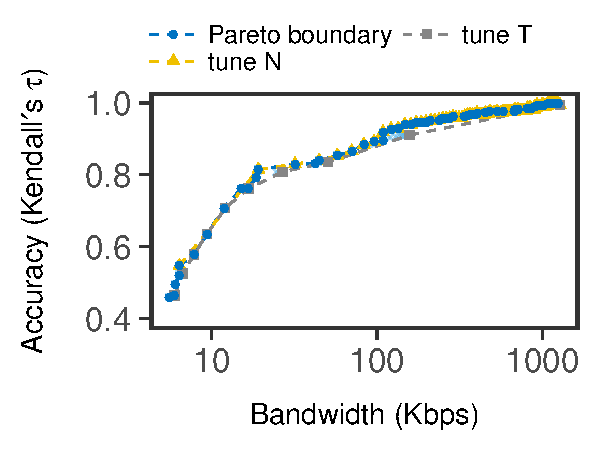
\includegraphics[width=\textwidth]{figures/profile-topk.pdf}
      \end{figure}
    \end{column}
    \begin{column}{0.55\textwidth}
      \begin{itemize}
        \visible<2->{
        \item The effect of each dimension is not significantly different.
        }
        \visible<3->{
        \item The profile offers quantified effects of degradation.
        }
      \end{itemize}
    \end{column}
  \end{columns}
\end{frame}

\begin{frame}{Evaluation: Runtime Experiment Baselines}
  \vspace{1em}
  \only<1-4>{
  \begin{table}
    \footnotesize
    \centering
    \begin{tabular}{ c m{0.6\linewidth} }
      \toprule
      \textbf{Baseline} & \textbf{Description} \\
      \midrule
      Streaming over TCP & A non-adaptive approach \\
      \midrule
      Streaming over UDP & A non-adaptive approach, represents RTP/UDP/RTSP
                           video streaming \\
      \midrule
      \visible<2->{
      \specialcell{JetStream\\\cite{rabkin2014aggregation}}
                        & Manual Policy: \textit{``if bandwidth is insufficient, switch to
                          sending images at 75\% fidelity, then 50\% if there still isn't enough
                          bandwidth. Beyond that point, reduce the frame rate, but keep the image
                          fidelity.''} \\
      \midrule
      }
      \visible<3->{
      JetStream++ & Uses adaptation policy generated by AWStream. JetStream
                    runtime does not probe (hence may oscillate between policies). \\
      \midrule
      }
      \visible<4->{
      \specialcell{HLS\\\cite{pantos2016http}}
                        & HTTP Live Streaming represents popular adaptive video
                          streaming techniques; used for Periscope video stream~\cite{wang2016anatomy}. \\
      \bottomrule
      }
    \end{tabular}
  \end{table}
  }

  \only<5->{
    \begin{figure}
      \centering
      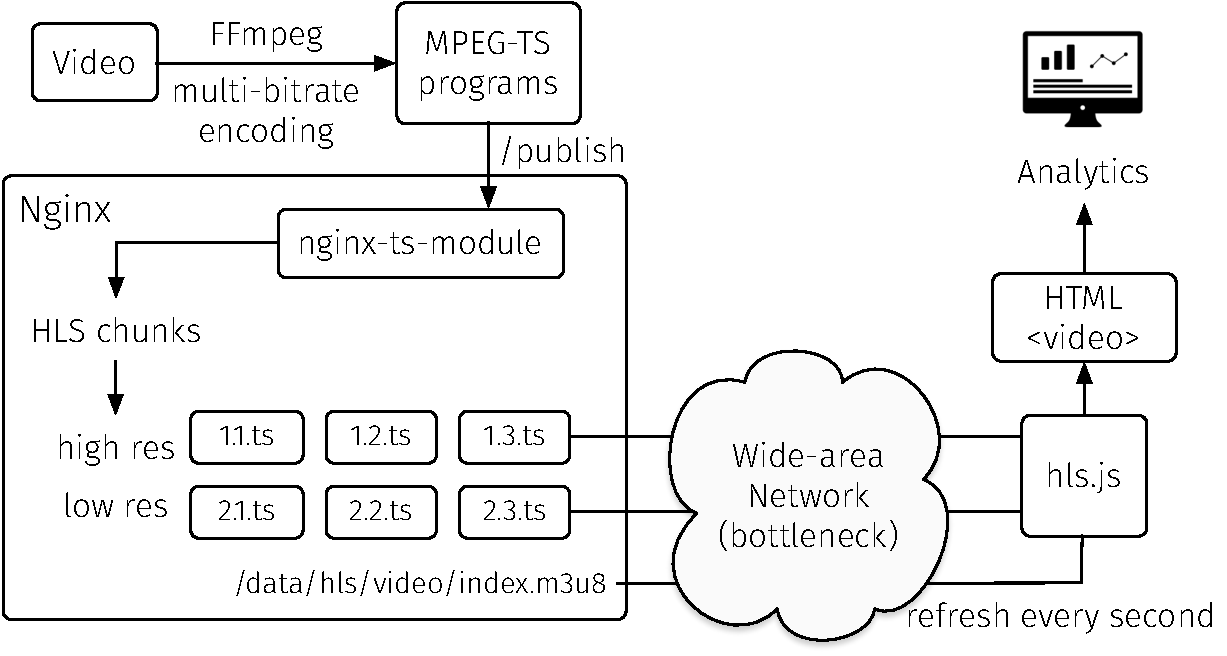
\includegraphics[width=0.8\textwidth]{figures/hls.pdf}
      \caption{HTTP Live Streaming (HLS) architecture: designed for live video
        viewing and relying on buffering at the viewing side.}
    \end{figure}
  }
\end{frame}

\begin{frame}{Evaluation: Runtime Performance}
  \only<1-5>{
    \begin{figure}
      \centering
      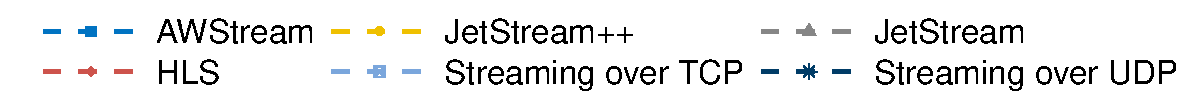
\includegraphics[width=0.8\textwidth]{figures/runtime-timeseries-legend.pdf}
    \end{figure}
    \vspace{-1em}
  }
  \only<1>{
    \begin{figure}
      \centering
      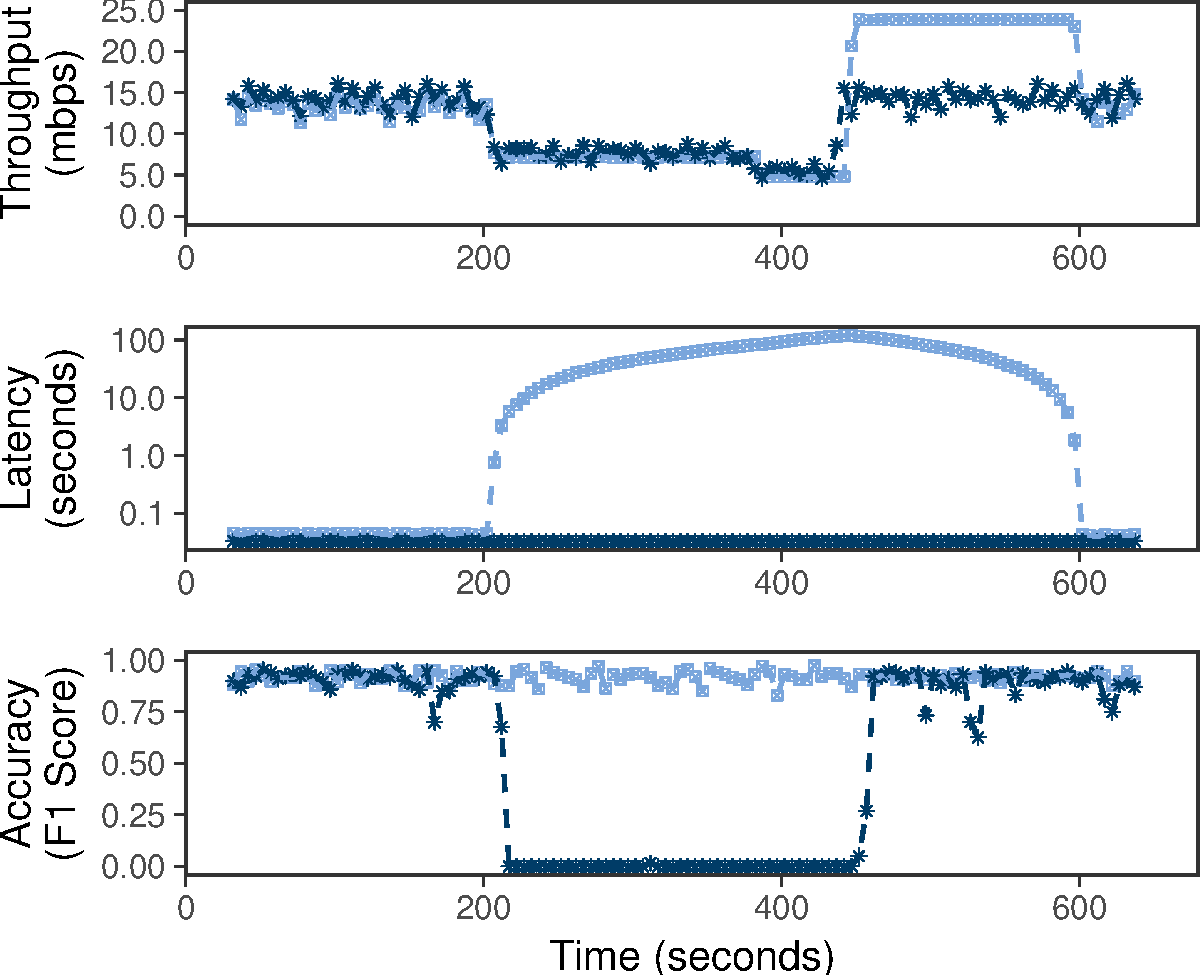
\includegraphics[width=0.8\textwidth]{figures/runtime-timeseries-1.pdf}
    \end{figure}
  }
  \only<2>{
    \begin{figure}
      \centering
      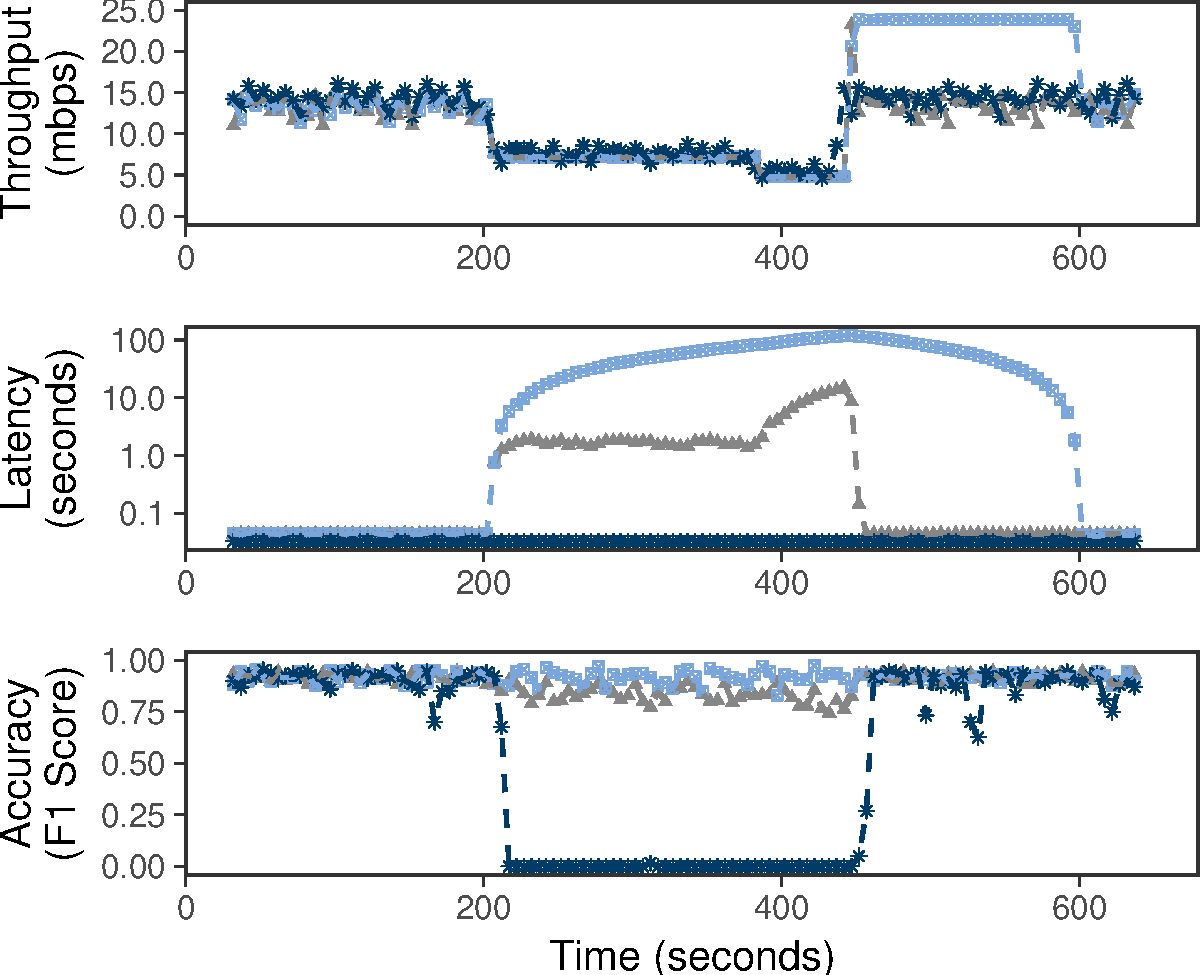
\includegraphics[width=0.8\textwidth]{figures/runtime-timeseries-2.pdf}
    \end{figure}
  }
  \only<3>{
    \begin{figure}
      \centering
      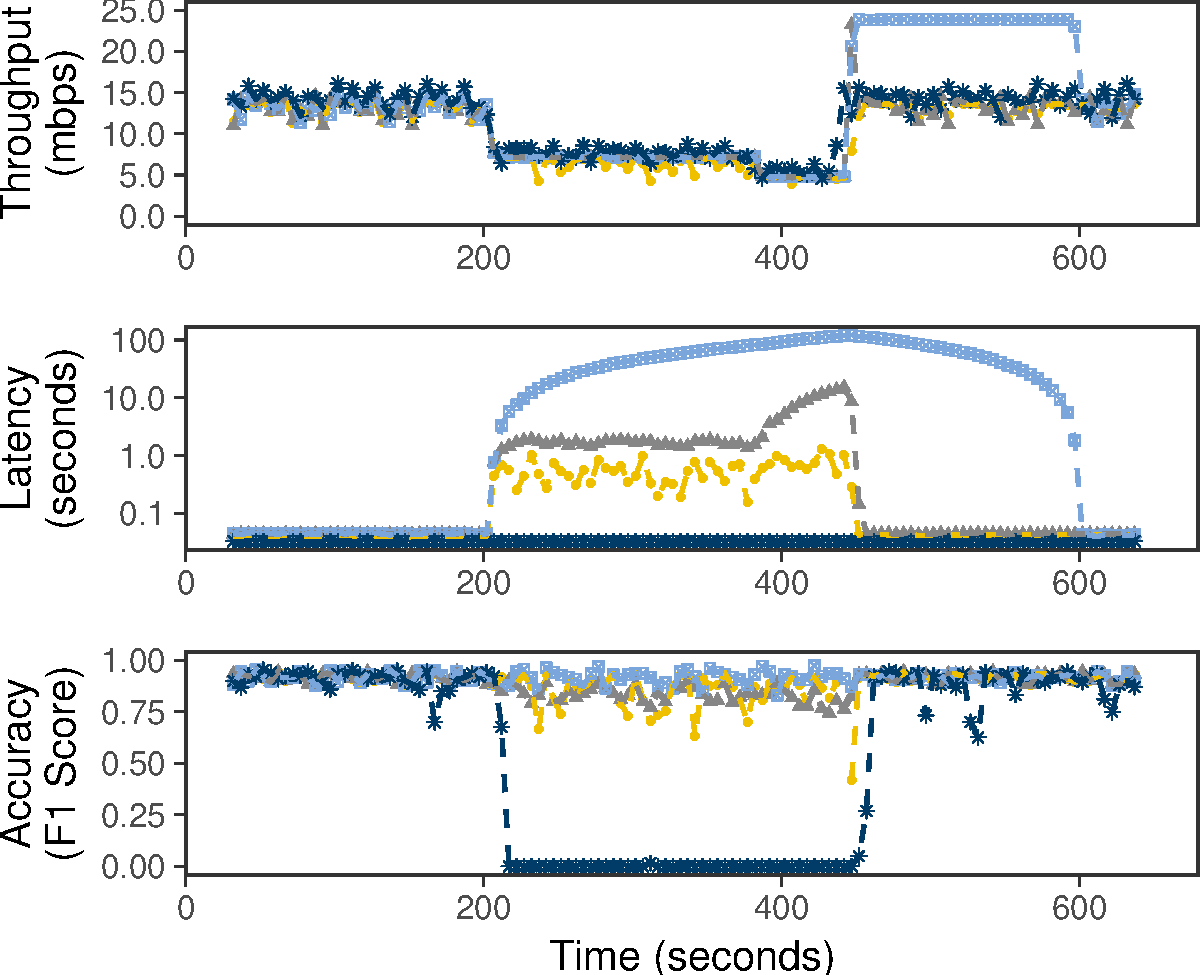
\includegraphics[width=0.8\textwidth]{figures/runtime-timeseries-3.pdf}
    \end{figure}
  }
  \only<4>{
    \begin{figure}
      \centering
      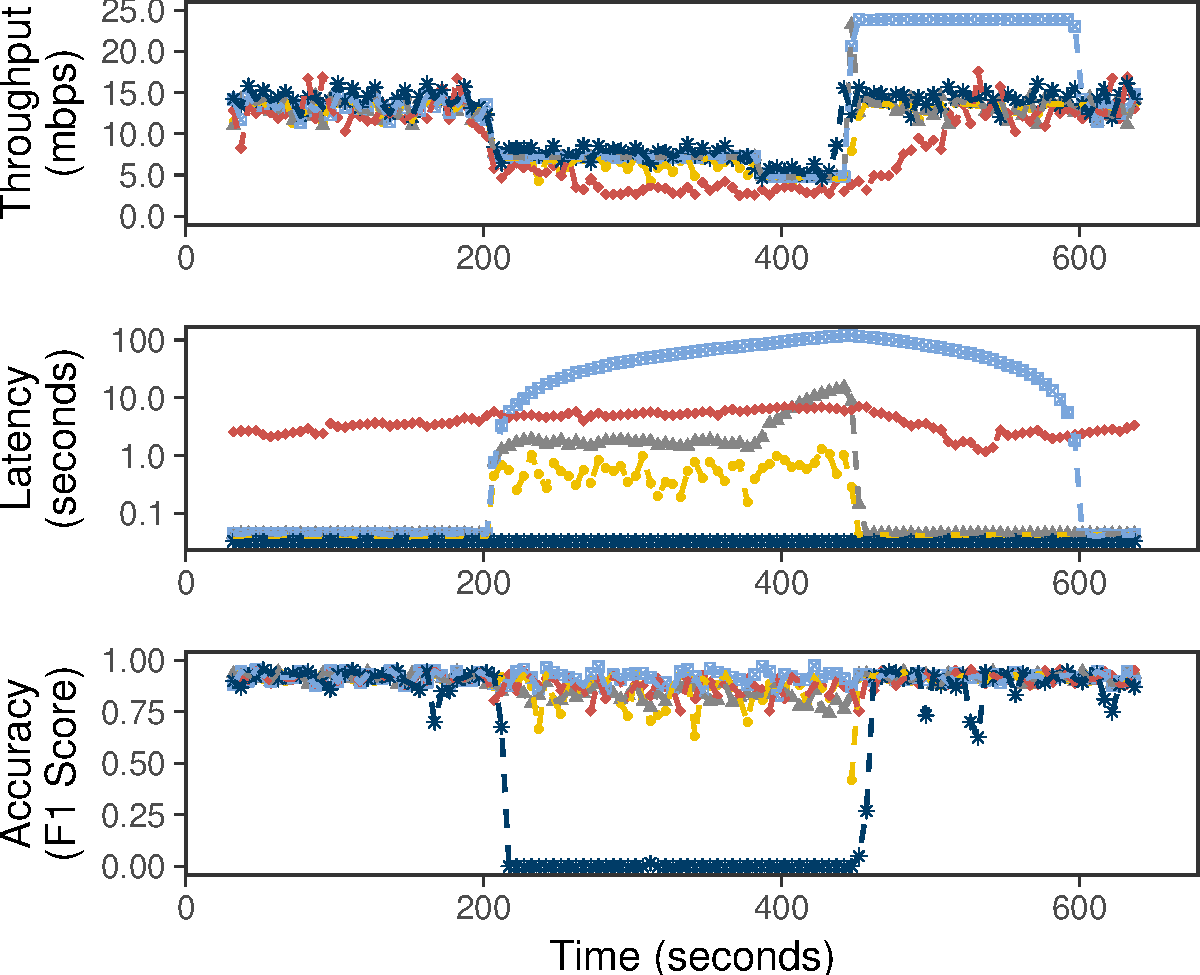
\includegraphics[width=0.8\textwidth]{figures/runtime-timeseries-4.pdf}
    \end{figure}
  }
  \only<5>{
    \begin{figure}
      \centering
      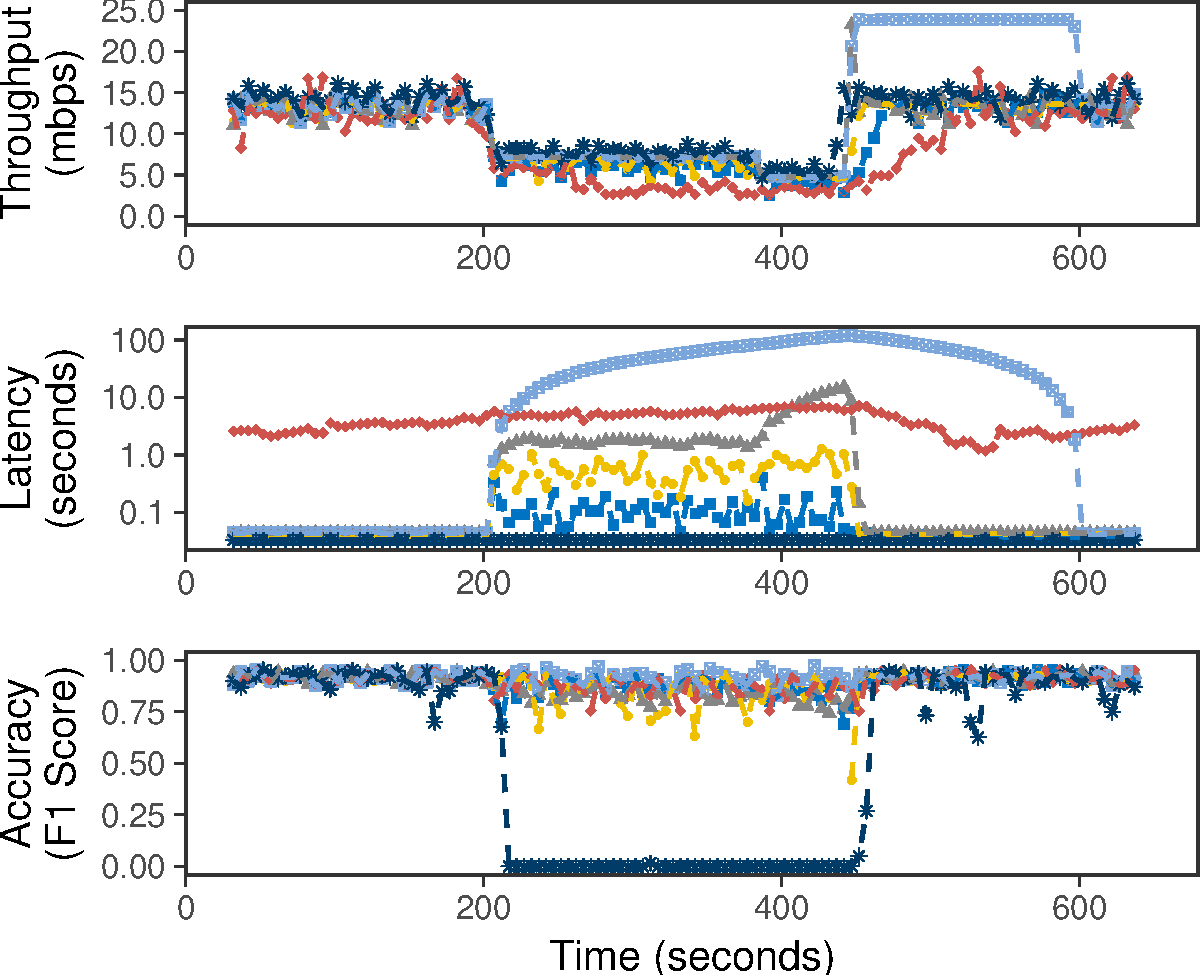
\includegraphics[width=0.8\textwidth]{figures/runtime-timeseries-5.pdf}
    \end{figure}
  }

  \only<6->{
    \begin{figure}
      \centering
      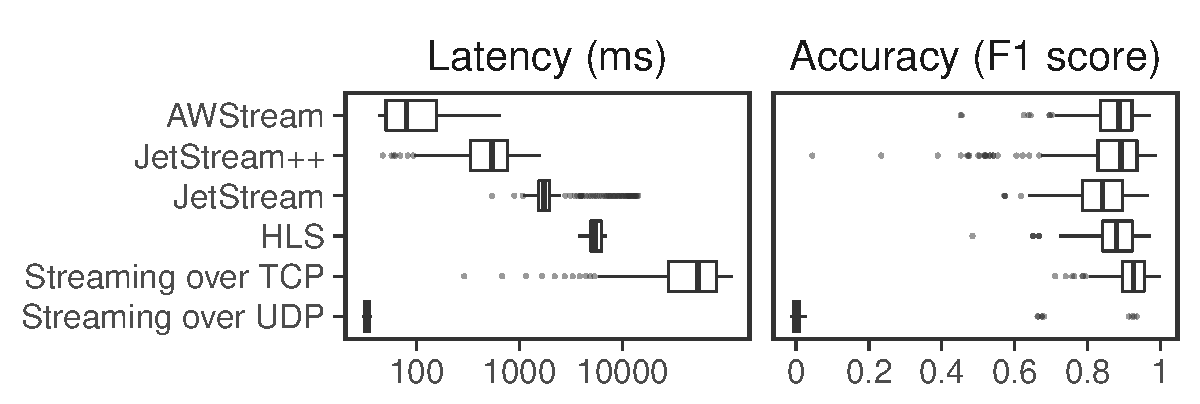
\includegraphics[width=0.8\textwidth]{figures/runtime-boxplot.pdf} \\
      \vspace{1em}
      \visible<7>{
        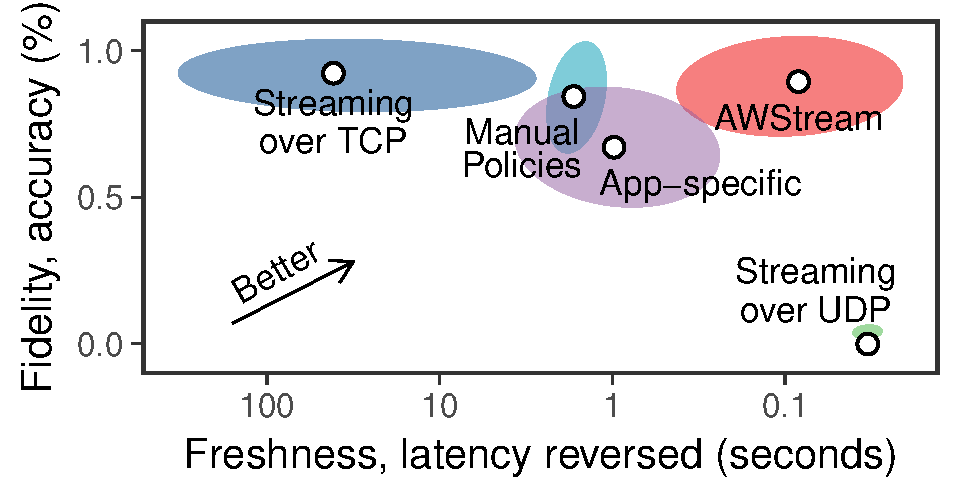
\includegraphics[width=0.6\columnwidth]{figures/fidelity-freshness-full.pdf}
      }
    \end{figure}
  }
\end{frame}

%%% Local Variables:
%%% mode: latex
%%% TeX-master: "../talk"
%%% TeX-engine: xetex
%%% End:

% \section{Epilogue}

\begin{frame}{Lessons \& Philosophy: Adaptation in Life}
  \centering
  \vspace{3em}
  \begin{tikzpicture}
    \draw [thick] [<->] (0,6) node [left] {Happiness}
    -- (0,0) --
    (6,0) node [below] {Money};

    \foreach \Point in {(5.5, 5.5), (5, 5.2), (4.5, 4.9), (4, 4.5), (3.8, 4.3)}{
      % \node<+-> [ACMBlue] at \Point {x};
      \node [ACMBlue] at \Point {x};
    }
  \end{tikzpicture}
\end{frame}

\begin{frame}{Acknowledgment}

  \begin{figure}
    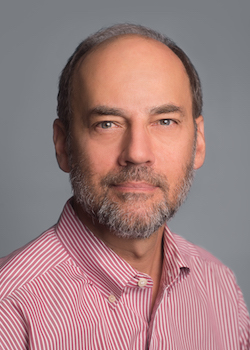
\includegraphics[width=0.15\linewidth]{figures/lee.jpg}
    \pause
    \hfill
    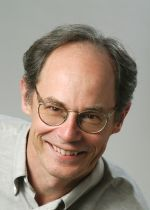
\includegraphics[width=0.15\linewidth]{figures/wawrzynek.jpg}
    \hfill
    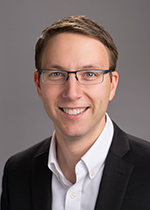
\includegraphics[width=0.15\linewidth]{figures/hartmann.jpg}
    \hfill
    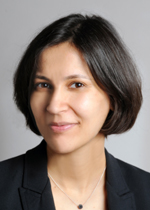
\includegraphics[width=0.15\linewidth]{figures/ratnasamy.jpg}
    \hfill
    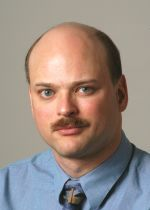
\includegraphics[width=0.15\linewidth]{figures/kubiatowicz.jpg}
    \hfill
  \end{figure}

  \begin{columns}
    \column{0.15\textwidth}
    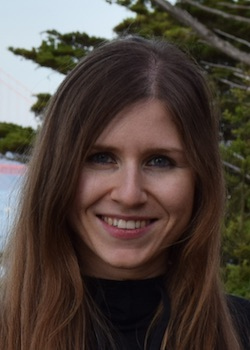
\includegraphics[width=0.9\linewidth]{figures/akkaya.jpg}
    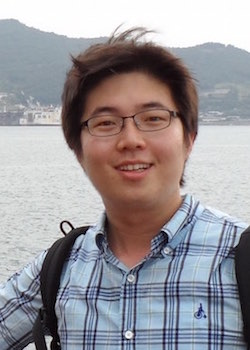
\includegraphics[width=0.9\linewidth]{figures/kim.jpg}

    \column{0.15\textwidth}
    \includegraphics[width=0.9\linewidth]{figures/shaver.jpg}
    \includegraphics[width=0.9\linewidth]{figures/iannopollo.jpg}

    \column{0.7\textwidth}
    \includegraphics[width=0.9\linewidth]{figures/ptolemy_group.jpg}
  \end{columns}

\end{frame}

\begin{frame}{Acknowledgement}
  \footnotesize \textcolor{ACMRed}{\heartpar{Edward Lee, John Wawrzynek, Syliva
      Ratnasamy, John Chuang, Bj\"orn Hartmann, John Kubiatowicz, Lin Zhang,
      David Mellis, Xin Jin, Mary Stewart, Christopher Brooks, Eunsuk Kang, Ilge
      Akkaya, Hokeun Kim, Marten Lohstroh, Matt Weber, Antonio Iannopollo,
      Mehrdad Niknami, Chris Shaver (Yvan Vivid), Michael Zimmer, Christos
      Stergiou, Dai Bui, Ben Lickly, Eleftherios Matsikoudis, Joseph Ng, Chadlia
      Jerad Ep Ben Haj Hmida, Moez Ben Haj Hmida, Maryam Bagheri, Victor
      Nouvellet, Ankush Desai, Nitesh Mor, Yu-Hsiang Sean Chen, Claire Tuna,
      Achal Dave, Jack Kolb, Eric Allman, Roy Wang, Bill N. Schilit, Jin Liang,
      Chao Mei, Kaifei Chen, Qifan Pu, Xiang Gao, Peihan Miao, Zhuo Chen, Yuting
      Wei, Chaoran Guo, Qian Zhong, Tianshi Wang}}
\end{frame}

%%% Local Variables:
%%% mode: latex
%%% TeX-master: "talk"
%%% TeX-engine: xetex
%%% End:


\fi

{
  \metroset{titleformat frame=allsmallcaps}
  \begin{frame}[allowframebreaks]{References}
    \scriptsize
    \bibliographystyle{apalike}
    \bibliography{talk}
  \end{frame}
}

\end{document}

%%% Local Variables:
%%% mode: latex
%%% TeX-master: t
%%% TeX-engine: xetex
%%% End:
